%%%%%%%%%%%%%%%%%%%%%%%%%%%%%%%%%%%%%%%%%
% Masters/Doctoral Thesis 
% LaTeX Template
% Version 2.5 (27/8/17)
%
% This template was downloaded from:
% http://www.LaTeXTemplates.com
%
% Version 2.x major modifications by:
% Vel (vel@latextemplates.com)
%
% This template is based on a template by:
% Steve Gunn (http://users.ecs.soton.ac.uk/srg/softwaretools/document/templates/)
% Sunil Patel (http://www.sunilpatel.co.uk/thesis-template/)
%
% Template license:
% CC BY-NC-SA 3.0 (http://creativecommons.org/licenses/by-nc-sa/3.0/)
%
%%%%%%%%%%%%%%%%%%%%%%%%%%%%%%%%%%%%%%%%%

%----------------------------------------------------------------------------------------
%	PACKAGES AND OTHER DOCUMENT CONFIGURATIONS
%----------------------------------------------------------------------------------------

\documentclass[
11pt, % The default document font size, options: 10pt, 11pt, 12pt
%oneside, % Two side (alternating margins) for binding by default, uncomment to switch to one side
english, % ngerman for German
singlespacing, % Single line spacing, alternatives: onehalfspacing or doublespacing
%draft, % Uncomment to enable draft mode (no pictures, no links, overfull hboxes indicated)
%nolistspacing, % If the document is onehalfspacing or doublespacing, uncomment this to set spacing in lists to single
%liststotoc, % Uncomment to add the list of figures/tables/etc to the table of contents
%toctotoc, % Uncomment to add the main table of contents to the table of contents
%parskip, % Uncomment to add space between paragraphs
%nohyperref, % Uncomment to not load the hyperref package
headsepline, % Uncomment to get a line under the header
%chapterinoneline, % Uncomment to place the chapter title next to the number on one line
%consistentlayout, % Uncomment to change the layout of the declaration, abstract and acknowledgements pages to match the default layout
]{MastersDoctoralThesis} % The class file specifying the document structure

\usepackage[utf8]{inputenc} % Required for inputting international characters
\usepackage[T1]{fontenc} % Output font encoding for international characters

\usepackage{mathpazo} % Use the Palatino font by default

\usepackage[backend=bibtex,style=authoryear,natbib=true]{biblatex} % Use the bibtex backend with the authoryear citation style (which resembles APA)

\addbibresource{example.bib} % The filename of the bibliography

\usepackage[autostyle=true]{csquotes} % Required to generate language-dependent quotes in the bibliography

\newcommand{\E}{\mathbb{E}}
\newcommand{\N}{\mathbb{N}}
\newcommand{\R}{\mathbb{R}}

\newcommand{\C}{\mathbf{C}}
\newcommand{\X}{\mathbf{X}}
\newcommand{\Z}{\mathbf{Z}}
\newcommand{\W}{\mathbf{W}}
\newcommand{\K}{\mathbf{K}}
\newcommand{\T}{\mathbf{T}}

\newcommand{\w}{\mathbf{w}}
\newcommand{\p}{\mathbf{p}}
\newcommand{\f}{\bm{f}}

\newcommand{\A}{\mathbf{A}}
\newcommand{\B}{\mathbf{B}}
\newcommand{\V}{\mathbf{V}}

\newcommand{\Pb}{\mathbf{P}}
\newcommand{\Qb}{\mathbf{Q}}
\newcommand{\Lb}{\mathbf{L}}

\newcommand{\varepsilonb}{\boldsymbol{\varepsilon}}
\newcommand{\gammab}{\boldsymbol{\gamma}}
\newcommand{\lambdab}{\boldsymbol{\lambda}}
\newcommand{\alphab}{\boldsymbol{\alpha}}
\newcommand{\betab}{\boldsymbol{\beta}}

\newcommand{\D}{\mathbf{D}}
\newcommand{\ind}{1\!\!1}

\newcommand{\eg}{\textit{e.g.}\ }
\newcommand{\ie}{\textit{i.e.}\ }

\newcommand{\KL}{\operatorname{KL}}
\newcommand{\diag}{\operatorname{diag}}

\newcommand{\Q}[1]{{\color{red}\bf #1}}

\newcommand{\integ}[1]{{[\![#1]\!]}}

% Recommended, but optional, packages for figures and better typesetting:
\usepackage{microtype}
\usepackage{graphicx}
\usepackage{subfigure}
\usepackage{booktabs} % for professional tables
\usepackage{hyperref}

% For theorems and such
\usepackage{amsmath}
\usepackage{amssymb}
\usepackage{mathtools}
\usepackage{amsthm}

%added packages 
\usepackage{bm}
\usepackage{bbm}
\usepackage{scalerel}
\usepackage{tikz}
\usepackage{nicematrix}
\usetikzlibrary{positioning}
\usepackage{xcolor,colortbl}
\usepackage{lmodern}
\usepackage{tablefootnote}
\usepackage{microtype}
\usepackage{graphicx}
\usepackage{subfigure}
\usepackage{booktabs}
\usepackage{hyperref}
\usepackage{cleveref}
\usepackage{amssymb}
\usepackage{algorithm,algorithmic}
\usepackage{wrapfig}

% Theorem, Lemma, etc
\theoremstyle{plain}
\newtheorem{theorem}{Theorem}
\newtheorem{corollary}[theorem]{Corollary}
\newtheorem{lemma}[theorem]{Lemma}
\newtheorem{claim}{Claim}[theorem]
\newtheorem{axiom}[theorem]{Axiom}
\newtheorem{conjecture}[theorem]{Conjecture}
\newtheorem{fact}[theorem]{Fact}
\newtheorem{hypothesis}[theorem]{Hypothesis}
\newtheorem{assumption}[theorem]{Assumption}
\newtheorem{proposition}[theorem]{Proposition}
\newtheorem{criterion}[theorem]{Criterion}
\theoremstyle{definition}
\newtheorem{definition}[theorem]{Definition}
\newtheorem{example}[theorem]{Example}
\newtheorem{remark}[theorem]{Remark}
\newtheorem{problem}[theorem]{Problem}
\newtheorem{principle}[theorem]{Principle}





%----------------------------------------------------------------------------------------
%	MARGIN SETTINGS
%----------------------------------------------------------------------------------------

\geometry{
	paper=a4paper, % Change to letterpaper for US letter
	inner=2.5cm, % Inner margin
	outer=3.8cm, % Outer margin
	bindingoffset=.5cm, % Binding offset
	top=1.5cm, % Top margin
	bottom=1.5cm, % Bottom margin
	%showframe, % Uncomment to show how the type block is set on the page
}

%----------------------------------------------------------------------------------------
%	THESIS INFORMATION
%----------------------------------------------------------------------------------------

\thesistitle{Thesis Title} % Your thesis title, this is used in the title and abstract, print it elsewhere with \ttitle
\supervisor{Dr. James \textsc{Smith}} % Your supervisor's name, this is used in the title page, print it elsewhere with \supname
\examiner{} % Your examiner's name, this is not currently used anywhere in the template, print it elsewhere with \examname
\degree{Doctor of Philosophy} % Your degree name, this is used in the title page and abstract, print it elsewhere with \degreename
\author{John \textsc{Smith}} % Your name, this is used in the title page and abstract, print it elsewhere with \authorname
\addresses{} % Your address, this is not currently used anywhere in the template, print it elsewhere with \addressname

\subject{Biological Sciences} % Your subject area, this is not currently used anywhere in the template, print it elsewhere with \subjectname
\keywords{} % Keywords for your thesis, this is not currently used anywhere in the template, print it elsewhere with \keywordnames
\university{\href{http://www.university.com}{University Name}} % Your university's name and URL, this is used in the title page and abstract, print it elsewhere with \univname
\department{\href{http://department.university.com}{Department or School Name}} % Your department's name and URL, this is used in the title page and abstract, print it elsewhere with \deptname
\group{\href{http://researchgroup.university.com}{Research Group Name}} % Your research group's name and URL, this is used in the title page, print it elsewhere with \groupname
\faculty{\href{http://faculty.university.com}{Faculty Name}} % Your faculty's name and URL, this is used in the title page and abstract, print it elsewhere with \facname

\AtBeginDocument{
\hypersetup{pdftitle=\ttitle} % Set the PDF's title to your title
\hypersetup{pdfauthor=\authorname} % Set the PDF's author to your name
\hypersetup{pdfkeywords=\keywordnames} % Set the PDF's keywords to your keywords
}

\begin{document}

\frontmatter % Use roman page numbering style (i, ii, iii, iv...) for the pre-content pages

\pagestyle{plain} % Default to the plain heading style until the thesis style is called for the body content

%----------------------------------------------------------------------------------------
%	TITLE PAGE
%----------------------------------------------------------------------------------------

\begin{titlepage}
\begin{center}

\vspace*{.06\textheight}
{\scshape\LARGE \univname\par}\vspace{1.5cm} % University name
\textsc{\Large Doctoral Thesis}\\[0.5cm] % Thesis type

\HRule \\[0.4cm] % Horizontal line
{\huge \bfseries \ttitle\par}\vspace{0.4cm} % Thesis title
\HRule \\[1.5cm] % Horizontal line
 
\begin{minipage}[t]{0.4\textwidth}
\begin{flushleft} \large
\emph{Author:}\\
\href{http://www.johnsmith.com}{\authorname} % Author name - remove the \href bracket to remove the link
\end{flushleft}
\end{minipage}
\begin{minipage}[t]{0.4\textwidth}
\begin{flushright} \large
\emph{Supervisor:} \\
\href{http://www.jamessmith.com}{\supname} % Supervisor name - remove the \href bracket to remove the link  
\end{flushright}
\end{minipage}\\[3cm]
 
\vfill

\large \textit{A thesis submitted in fulfillment of the requirements\\ for the degree of \degreename}\\[0.3cm] % University requirement text
\textit{in the}\\[0.4cm]
\groupname\\\deptname\\[2cm] % Research group name and department name
 
\vfill

{\large \today}\\[4cm] % Date
%\includegraphics{Logo} % University/department logo - uncomment to place it
 
\vfill
\end{center}
\end{titlepage}

%----------------------------------------------------------------------------------------
%	DECLARATION PAGE
%----------------------------------------------------------------------------------------

\begin{declaration}
\addchaptertocentry{\authorshipname} % Add the declaration to the table of contents
\noindent I, \authorname, declare that this thesis titled, \enquote{\ttitle} and the work presented in it are my own. I confirm that:

\begin{itemize} 
\item This work was done wholly or mainly while in candidature for a research degree at this University.
\item Where any part of this thesis has previously been submitted for a degree or any other qualification at this University or any other institution, this has been clearly stated.
\item Where I have consulted the published work of others, this is always clearly attributed.
\item Where I have quoted from the work of others, the source is always given. With the exception of such quotations, this thesis is entirely my own work.
\item I have acknowledged all main sources of help.
\item Where the thesis is based on work done by myself jointly with others, I have made clear exactly what was done by others and what I have contributed myself.\\
\end{itemize}
 
\noindent Signed:\\
\rule[0.5em]{25em}{0.5pt} % This prints a line for the signature
 
\noindent Date:\\
\rule[0.5em]{25em}{0.5pt} % This prints a line to write the date
\end{declaration}

\cleardoublepage

%----------------------------------------------------------------------------------------
%	QUOTATION PAGE
%----------------------------------------------------------------------------------------

\vspace*{0.2\textheight}

\noindent\enquote{\itshape Thanks to my solid academic training, today I can write hundreds of words on virtually any topic without possessing a shred of information, which is how I got a good job in journalism.}\bigbreak

\hfill Dave Barry

%----------------------------------------------------------------------------------------
%	ABSTRACT PAGE
%----------------------------------------------------------------------------------------

\begin{abstract}
\addchaptertocentry{\abstractname} % Add the abstract to the table of contents
The Thesis Abstract is written here (and usually kept to just this page). The page is kept centered vertically so can expand into the blank space above the title too\ldots
\end{abstract}

%----------------------------------------------------------------------------------------
%	ACKNOWLEDGEMENTS
%----------------------------------------------------------------------------------------

\begin{acknowledgements}
\addchaptertocentry{\acknowledgementname} % Add the acknowledgements to the table of contents
The acknowledgments and the people to thank go here, don't forget to include your project advisor\ldots
\end{acknowledgements}

%----------------------------------------------------------------------------------------
%	LIST OF CONTENTS/FIGURES/TABLES PAGES
%----------------------------------------------------------------------------------------

\tableofcontents % Prints the main table of contents

\listoffigures % Prints the list of figures

\listoftables % Prints the list of tables

%----------------------------------------------------------------------------------------
%	ABBREVIATIONS
%----------------------------------------------------------------------------------------

\begin{abbreviations}{ll} % Include a list of abbreviations (a table of two columns)

\textbf{LAH} & \textbf{L}ist \textbf{A}bbreviations \textbf{H}ere\\
\textbf{WSF} & \textbf{W}hat (it) \textbf{S}tands \textbf{F}or\\

\end{abbreviations}

%----------------------------------------------------------------------------------------
%	PHYSICAL CONSTANTS/OTHER DEFINITIONS
%----------------------------------------------------------------------------------------

\begin{constants}{lr@{${}={}$}l} % The list of physical constants is a three column table

% The \SI{}{} command is provided by the siunitx package, see its documentation for instructions on how to use it

Speed of Light & $c_{0}$ & \SI{2.99792458e8}{\meter\per\second} (exact)\\
%Constant Name & $Symbol$ & $Constant Value$ with units\\

\end{constants}

%----------------------------------------------------------------------------------------
%	SYMBOLS
%----------------------------------------------------------------------------------------

\begin{symbols}{lll} % Include a list of Symbols (a three column table)

$a$ & distance & \si{\meter} \\
$P$ & power & \si{\watt} (\si{\joule\per\second}) \\
%Symbol & Name & Unit \\

\addlinespace % Gap to separate the Roman symbols from the Greek

$\omega$ & angular frequency & \si{\radian} \\

\end{symbols}

%----------------------------------------------------------------------------------------
%	DEDICATION
%----------------------------------------------------------------------------------------

\dedicatory{For/Dedicated to/To my\ldots} 

%----------------------------------------------------------------------------------------
%	THESIS CONTENT - CHAPTERS
%----------------------------------------------------------------------------------------

\mainmatter % Begin numeric (1,2,3...) page numbering

\pagestyle{thesis} % Return the page headers back to the "thesis" style

% Include the chapters of the thesis as separate files from the Chapters folder
% Uncomment the lines as you write the chapters

% Chapter 1

\chapter{Chapter Title Here} % Main chapter title

\label{Chapter1} % For referencing the chapter elsewhere, use \ref{Chapter1} 

%----------------------------------------------------------------------------------------

% Define some commands to keep the formatting separated from the content 
\newcommand{\keyword}[1]{\textbf{#1}}
\newcommand{\tabhead}[1]{\textbf{#1}}
\newcommand{\code}[1]{\texttt{#1}}
\newcommand{\file}[1]{\texttt{\bfseries#1}}
\newcommand{\option}[1]{\texttt{\itshape#1}}

%----------------------------------------------------------------------------------------

\section{Welcome and Thank You}
Welcome to this \LaTeX{} Thesis Template, a beautiful and easy to use template for writing a thesis using the \LaTeX{} typesetting system.

If you are writing a thesis (or will be in the future) and its subject is technical or mathematical (though it doesn't have to be), then creating it in \LaTeX{} is highly recommended as a way to make sure you can just get down to the essential writing without having to worry over formatting or wasting time arguing with your word processor.

\LaTeX{} is easily able to professionally typeset documents that run to hundreds or thousands of pages long. With simple mark-up commands, it automatically sets out the table of contents, margins, page headers and footers and keeps the formatting consistent and beautiful. One of its main strengths is the way it can easily typeset mathematics, even \emph{heavy} mathematics. Even if those equations are the most horribly twisted and most difficult mathematical problems that can only be solved on a super-computer, you can at least count on \LaTeX{} to make them look stunning.

%----------------------------------------------------------------------------------------

\section{Learning \LaTeX{}}

\LaTeX{} is not a \textsc{wysiwyg} (What You See is What You Get) program, unlike word processors such as Microsoft Word or Apple's Pages. Instead, a document written for \LaTeX{} is actually a simple, plain text file that contains \emph{no formatting}. You tell \LaTeX{} how you want the formatting in the finished document by writing in simple commands amongst the text, for example, if I want to use \emph{italic text for emphasis}, I write the \verb|\emph{text}| command and put the text I want in italics in between the curly braces. This means that \LaTeX{} is a \enquote{mark-up} language, very much like HTML.

\subsection{A (not so short) Introduction to \LaTeX{}}

If you are new to \LaTeX{}, there is a very good eBook -- freely available online as a PDF file -- called, \enquote{The Not So Short Introduction to \LaTeX{}}. The book's title is typically shortened to just \emph{lshort}. You can download the latest version (as it is occasionally updated) from here:
\url{http://www.ctan.org/tex-archive/info/lshort/english/lshort.pdf}

It is also available in several other languages. Find yours from the list on this page: \url{http://www.ctan.org/tex-archive/info/lshort/}

It is recommended to take a little time out to learn how to use \LaTeX{} by creating several, small `test' documents, or having a close look at several templates on:\\ 
\url{http://www.LaTeXTemplates.com}\\ 
Making the effort now means you're not stuck learning the system when what you \emph{really} need to be doing is writing your thesis.

\subsection{A Short Math Guide for \LaTeX{}}

If you are writing a technical or mathematical thesis, then you may want to read the document by the AMS (American Mathematical Society) called, \enquote{A Short Math Guide for \LaTeX{}}. It can be found online here:
\url{http://www.ams.org/tex/amslatex.html}
under the \enquote{Additional Documentation} section towards the bottom of the page.

\subsection{Common \LaTeX{} Math Symbols}
There are a multitude of mathematical symbols available for \LaTeX{} and it would take a great effort to learn the commands for them all. The most common ones you are likely to use are shown on this page:
\url{http://www.sunilpatel.co.uk/latex-type/latex-math-symbols/}

You can use this page as a reference or crib sheet, the symbols are rendered as large, high quality images so you can quickly find the \LaTeX{} command for the symbol you need.

\subsection{\LaTeX{} on a Mac}
 
The \LaTeX{} distribution is available for many systems including Windows, Linux and Mac OS X. The package for OS X is called MacTeX and it contains all the applications you need -- bundled together and pre-customized -- for a fully working \LaTeX{} environment and work flow.
 
MacTeX includes a custom dedicated \LaTeX{} editor called TeXShop for writing your `\file{.tex}' files and BibDesk: a program to manage your references and create your bibliography section just as easily as managing songs and creating playlists in iTunes.

%----------------------------------------------------------------------------------------

\section{Getting Started with this Template}

If you are familiar with \LaTeX{}, then you should explore the directory structure of the template and then proceed to place your own information into the \emph{THESIS INFORMATION} block of the \file{main.tex} file. You can then modify the rest of this file to your unique specifications based on your degree/university. Section \ref{FillingFile} on page \pageref{FillingFile} will help you do this. Make sure you also read section \ref{ThesisConventions} about thesis conventions to get the most out of this template.

If you are new to \LaTeX{} it is recommended that you carry on reading through the rest of the information in this document.

Before you begin using this template you should ensure that its style complies with the thesis style guidelines imposed by your institution. In most cases this template style and layout will be suitable. If it is not, it may only require a small change to bring the template in line with your institution's recommendations. These modifications will need to be done on the \file{MastersDoctoralThesis.cls} file.

\subsection{About this Template}

This \LaTeX{} Thesis Template is originally based and created around a \LaTeX{} style file created by Steve R.\ Gunn from the University of Southampton (UK), department of Electronics and Computer Science. You can find his original thesis style file at his site, here:
\url{http://www.ecs.soton.ac.uk/~srg/softwaretools/document/templates/}

Steve's \file{ecsthesis.cls} was then taken by Sunil Patel who modified it by creating a skeleton framework and folder structure to place the thesis files in. The resulting template can be found on Sunil's site here:
\url{http://www.sunilpatel.co.uk/thesis-template}

Sunil's template was made available through \url{http://www.LaTeXTemplates.com} where it was modified many times based on user requests and questions. Version 2.0 and onwards of this template represents a major modification to Sunil's template and is, in fact, hardly recognisable. The work to make version 2.0 possible was carried out by \href{mailto:vel@latextemplates.com}{Vel} and Johannes Böttcher.

%----------------------------------------------------------------------------------------

\section{What this Template Includes}

\subsection{Folders}

This template comes as a single zip file that expands out to several files and folders. The folder names are mostly self-explanatory:

\keyword{Appendices} -- this is the folder where you put the appendices. Each appendix should go into its own separate \file{.tex} file. An example and template are included in the directory.

\keyword{Chapters} -- this is the folder where you put the thesis chapters. A thesis usually has about six chapters, though there is no hard rule on this. Each chapter should go in its own separate \file{.tex} file and they can be split as:
\begin{itemize}
\item Chapter 1: Introduction to the thesis topic
\item Chapter 2: Background information and theory
\item Chapter 3: (Laboratory) experimental setup
\item Chapter 4: Details of experiment 1
\item Chapter 5: Details of experiment 2
\item Chapter 6: Discussion of the experimental results
\item Chapter 7: Conclusion and future directions
\end{itemize}
This chapter layout is specialised for the experimental sciences, your discipline may be different.

\keyword{Figures} -- this folder contains all figures for the thesis. These are the final images that will go into the thesis document.

\subsection{Files}

Included are also several files, most of them are plain text and you can see their contents in a text editor. After initial compilation, you will see that more auxiliary files are created by \LaTeX{} or BibTeX and which you don't need to delete or worry about:

\keyword{example.bib} -- this is an important file that contains all the bibliographic information and references that you will be citing in the thesis for use with BibTeX. You can write it manually, but there are reference manager programs available that will create and manage it for you. Bibliographies in \LaTeX{} are a large subject and you may need to read about BibTeX before starting with this. Many modern reference managers will allow you to export your references in BibTeX format which greatly eases the amount of work you have to do.

\keyword{MastersDoctoralThesis.cls} -- this is an important file. It is the class file that tells \LaTeX{} how to format the thesis. 

\keyword{main.pdf} -- this is your beautifully typeset thesis (in the PDF file format) created by \LaTeX{}. It is supplied in the PDF with the template and after you compile the template you should get an identical version.

\keyword{main.tex} -- this is an important file. This is the file that you tell \LaTeX{} to compile to produce your thesis as a PDF file. It contains the framework and constructs that tell \LaTeX{} how to layout the thesis. It is heavily commented so you can read exactly what each line of code does and why it is there. After you put your own information into the \emph{THESIS INFORMATION} block -- you have now started your thesis!

Files that are \emph{not} included, but are created by \LaTeX{} as auxiliary files include:

\keyword{main.aux} -- this is an auxiliary file generated by \LaTeX{}, if it is deleted \LaTeX{} simply regenerates it when you run the main \file{.tex} file.

\keyword{main.bbl} -- this is an auxiliary file generated by BibTeX, if it is deleted, BibTeX simply regenerates it when you run the \file{main.aux} file. Whereas the \file{.bib} file contains all the references you have, this \file{.bbl} file contains the references you have actually cited in the thesis and is used to build the bibliography section of the thesis.

\keyword{main.blg} -- this is an auxiliary file generated by BibTeX, if it is deleted BibTeX simply regenerates it when you run the main \file{.aux} file.

\keyword{main.lof} -- this is an auxiliary file generated by \LaTeX{}, if it is deleted \LaTeX{} simply regenerates it when you run the main \file{.tex} file. It tells \LaTeX{} how to build the \emph{List of Figures} section.

\keyword{main.log} -- this is an auxiliary file generated by \LaTeX{}, if it is deleted \LaTeX{} simply regenerates it when you run the main \file{.tex} file. It contains messages from \LaTeX{}, if you receive errors and warnings from \LaTeX{}, they will be in this \file{.log} file.

\keyword{main.lot} -- this is an auxiliary file generated by \LaTeX{}, if it is deleted \LaTeX{} simply regenerates it when you run the main \file{.tex} file. It tells \LaTeX{} how to build the \emph{List of Tables} section.

\keyword{main.out} -- this is an auxiliary file generated by \LaTeX{}, if it is deleted \LaTeX{} simply regenerates it when you run the main \file{.tex} file.

So from this long list, only the files with the \file{.bib}, \file{.cls} and \file{.tex} extensions are the most important ones. The other auxiliary files can be ignored or deleted as \LaTeX{} and BibTeX will regenerate them.

%----------------------------------------------------------------------------------------

\section{Filling in Your Information in the \file{main.tex} File}\label{FillingFile}

You will need to personalise the thesis template and make it your own by filling in your own information. This is done by editing the \file{main.tex} file in a text editor or your favourite LaTeX environment.

Open the file and scroll down to the third large block titled \emph{THESIS INFORMATION} where you can see the entries for \emph{University Name}, \emph{Department Name}, etc \ldots

Fill out the information about yourself, your group and institution. You can also insert web links, if you do, make sure you use the full URL, including the \code{http://} for this. If you don't want these to be linked, simply remove the \verb|\href{url}{name}| and only leave the name.

When you have done this, save the file and recompile \code{main.tex}. All the information you filled in should now be in the PDF, complete with web links. You can now begin your thesis proper!

%----------------------------------------------------------------------------------------

\section{The \code{main.tex} File Explained}

The \file{main.tex} file contains the structure of the thesis. There are plenty of written comments that explain what pages, sections and formatting the \LaTeX{} code is creating. Each major document element is divided into commented blocks with titles in all capitals to make it obvious what the following bit of code is doing. Initially there seems to be a lot of \LaTeX{} code, but this is all formatting, and it has all been taken care of so you don't have to do it.

Begin by checking that your information on the title page is correct. For the thesis declaration, your institution may insist on something different than the text given. If this is the case, just replace what you see with what is required in the \emph{DECLARATION PAGE} block.

Then comes a page which contains a funny quote. You can put your own, or quote your favourite scientist, author, person, and so on. Make sure to put the name of the person who you took the quote from.

Following this is the abstract page which summarises your work in a condensed way and can almost be used as a standalone document to describe what you have done. The text you write will cause the heading to move up so don't worry about running out of space.

Next come the acknowledgements. On this page, write about all the people who you wish to thank (not forgetting parents, partners and your advisor/supervisor).

The contents pages, list of figures and tables are all taken care of for you and do not need to be manually created or edited. The next set of pages are more likely to be optional and can be deleted since they are for a more technical thesis: insert a list of abbreviations you have used in the thesis, then a list of the physical constants and numbers you refer to and finally, a list of mathematical symbols used in any formulae. Making the effort to fill these tables means the reader has a one-stop place to refer to instead of searching the internet and references to try and find out what you meant by certain abbreviations or symbols.

The list of symbols is split into the Roman and Greek alphabets. Whereas the abbreviations and symbols ought to be listed in alphabetical order (and this is \emph{not} done automatically for you) the list of physical constants should be grouped into similar themes.

The next page contains a one line dedication. Who will you dedicate your thesis to?

Finally, there is the block where the chapters are included. Uncomment the lines (delete the \code{\%} character) as you write the chapters. Each chapter should be written in its own file and put into the \emph{Chapters} folder and named \file{Chapter1}, \file{Chapter2}, etc\ldots Similarly for the appendices, uncomment the lines as you need them. Each appendix should go into its own file and placed in the \emph{Appendices} folder.

After the preamble, chapters and appendices finally comes the bibliography. The bibliography style (called \option{authoryear}) is used for the bibliography and is a fully featured style that will even include links to where the referenced paper can be found online. Do not underestimate how grateful your reader will be to find that a reference to a paper is just a click away. Of course, this relies on you putting the URL information into the BibTeX file in the first place.

%----------------------------------------------------------------------------------------

\section{Thesis Features and Conventions}\label{ThesisConventions}

To get the best out of this template, there are a few conventions that you may want to follow.

One of the most important (and most difficult) things to keep track of in such a long document as a thesis is consistency. Using certain conventions and ways of doing things (such as using a Todo list) makes the job easier. Of course, all of these are optional and you can adopt your own method.

\subsection{Printing Format}

This thesis template is designed for double sided printing (i.e. content on the front and back of pages) as most theses are printed and bound this way. Switching to one sided printing is as simple as uncommenting the \option{oneside} option of the \code{documentclass} command at the top of the \file{main.tex} file. You may then wish to adjust the margins to suit specifications from your institution.

The headers for the pages contain the page number on the outer side (so it is easy to flick through to the page you want) and the chapter name on the inner side.

The text is set to 11 point by default with single line spacing, again, you can tune the text size and spacing should you want or need to using the options at the very start of \file{main.tex}. The spacing can be changed similarly by replacing the \option{singlespacing} with \option{onehalfspacing} or \option{doublespacing}.

\subsection{Using US Letter Paper}

The paper size used in the template is A4, which is the standard size in Europe. If you are using this thesis template elsewhere and particularly in the United States, then you may have to change the A4 paper size to the US Letter size. This can be done in the margins settings section in \file{main.tex}.

Due to the differences in the paper size, the resulting margins may be different to what you like or require (as it is common for institutions to dictate certain margin sizes). If this is the case, then the margin sizes can be tweaked by modifying the values in the same block as where you set the paper size. Now your document should be set up for US Letter paper size with suitable margins.

\subsection{References}

The \code{biblatex} package is used to format the bibliography and inserts references such as this one \parencite{Reference1}. The options used in the \file{main.tex} file mean that the in-text citations of references are formatted with the author(s) listed with the date of the publication. Multiple references are separated by semicolons (e.g. \parencite{Reference2, Reference1}) and references with more than three authors only show the first author with \emph{et al.} indicating there are more authors (e.g. \parencite{Reference3}). This is done automatically for you. To see how you use references, have a look at the \file{Chapter1.tex} source file. Many reference managers allow you to simply drag the reference into the document as you type.

Scientific references should come \emph{before} the punctuation mark if there is one (such as a comma or period). The same goes for footnotes\footnote{Such as this footnote, here down at the bottom of the page.}. You can change this but the most important thing is to keep the convention consistent throughout the thesis. Footnotes themselves should be full, descriptive sentences (beginning with a capital letter and ending with a full stop). The APA6 states: \enquote{Footnote numbers should be superscripted, [...], following any punctuation mark except a dash.} The Chicago manual of style states: \enquote{A note number should be placed at the end of a sentence or clause. The number follows any punctuation mark except the dash, which it precedes. It follows a closing parenthesis.}

The bibliography is typeset with references listed in alphabetical order by the first author's last name. This is similar to the APA referencing style. To see how \LaTeX{} typesets the bibliography, have a look at the very end of this document (or just click on the reference number links in in-text citations).

\subsubsection{A Note on bibtex}

The bibtex backend used in the template by default does not correctly handle unicode character encoding (i.e. "international" characters). You may see a warning about this in the compilation log and, if your references contain unicode characters, they may not show up correctly or at all. The solution to this is to use the biber backend instead of the outdated bibtex backend. This is done by finding this in \file{main.tex}: \option{backend=bibtex} and changing it to \option{backend=biber}. You will then need to delete all auxiliary BibTeX files and navigate to the template directory in your terminal (command prompt). Once there, simply type \code{biber main} and biber will compile your bibliography. You can then compile \file{main.tex} as normal and your bibliography will be updated. An alternative is to set up your LaTeX editor to compile with biber instead of bibtex, see \href{http://tex.stackexchange.com/questions/154751/biblatex-with-biber-configuring-my-editor-to-avoid-undefined-citations/}{here} for how to do this for various editors.

\subsection{Tables}

Tables are an important way of displaying your results, below is an example table which was generated with this code:

{\small
\begin{verbatim}
\begin{table}
\caption{The effects of treatments X and Y on the four groups studied.}
\label{tab:treatments}
\centering
\begin{tabular}{l l l}
\toprule
\tabhead{Groups} & \tabhead{Treatment X} & \tabhead{Treatment Y} \\
\midrule
1 & 0.2 & 0.8\\
2 & 0.17 & 0.7\\
3 & 0.24 & 0.75\\
4 & 0.68 & 0.3\\
\bottomrule\\
\end{tabular}
\end{table}
\end{verbatim}
}

\begin{table}
\caption{The effects of treatments X and Y on the four groups studied.}
\label{tab:treatments}
\centering
\begin{tabular}{l l l}
\toprule
\tabhead{Groups} & \tabhead{Treatment X} & \tabhead{Treatment Y} \\
\midrule
1 & 0.2 & 0.8\\
2 & 0.17 & 0.7\\
3 & 0.24 & 0.75\\
4 & 0.68 & 0.3\\
\bottomrule\\
\end{tabular}
\end{table}

You can reference tables with \verb|\ref{<label>}| where the label is defined within the table environment. See \file{Chapter1.tex} for an example of the label and citation (e.g. Table~\ref{tab:treatments}).

\subsection{Figures}

There will hopefully be many figures in your thesis (that should be placed in the \emph{Figures} folder). The way to insert figures into your thesis is to use a code template like this:
\begin{verbatim}
\begin{figure}
\centering

\includegraphics{Figures/Electron}
\decoRule
\caption[An Electron]{An electron (artist's impression).}
\label{fig:Electron}
\end{figure}
\end{verbatim}
Also look in the source file. Putting this code into the source file produces the picture of the electron that you can see in the figure below.

\begin{figure}[th]
\centering

\includegraphics{Figures/Electron}
\decoRule
\caption[An Electron]{An electron (artist's impression).}
\label{fig:Electron}
\end{figure}

Sometimes figures don't always appear where you write them in the source. The placement depends on how much space there is on the page for the figure. Sometimes there is not enough room to fit a figure directly where it should go (in relation to the text) and so \LaTeX{} puts it at the top of the next page. Positioning figures is the job of \LaTeX{} and so you should only worry about making them look good!

Figures usually should have captions just in case you need to refer to them (such as in Figure~\ref{fig:Electron}). The \verb|\caption| command contains two parts, the first part, inside the square brackets is the title that will appear in the \emph{List of Figures}, and so should be short. The second part in the curly brackets should contain the longer and more descriptive caption text.

The \verb|\decoRule| command is optional and simply puts an aesthetic horizontal line below the image. If you do this for one image, do it for all of them.

\LaTeX{} is capable of using images in pdf, jpg and png format.

\subsection{Typesetting mathematics}

If your thesis is going to contain heavy mathematical content, be sure that \LaTeX{} will make it look beautiful, even though it won't be able to solve the equations for you.

The \enquote{Not So Short Introduction to \LaTeX} (available on \href{http://www.ctan.org/tex-archive/info/lshort/english/lshort.pdf}{CTAN}) should tell you everything you need to know for most cases of typesetting mathematics. If you need more information, a much more thorough mathematical guide is available from the AMS called, \enquote{A Short Math Guide to \LaTeX} and can be downloaded from:
\url{ftp://ftp.ams.org/pub/tex/doc/amsmath/short-math-guide.pdf}

There are many different \LaTeX{} symbols to remember, luckily you can find the most common symbols in \href{http://ctan.org/pkg/comprehensive}{The Comprehensive \LaTeX~Symbol List}.

You can write an equation, which is automatically given an equation number by \LaTeX{} like this:
\begin{verbatim}
\begin{equation}
E = mc^{2}
\label{eqn:Einstein}
\end{equation}
\end{verbatim}

This will produce Einstein's famous energy-matter equivalence equation:
\begin{equation}
E = mc^{2}
\label{eqn:Einstein}
\end{equation}

All equations you write (which are not in the middle of paragraph text) are automatically given equation numbers by \LaTeX{}. If you don't want a particular equation numbered, use the unnumbered form:
\begin{verbatim}
\[ a^{2}=4 \]
\end{verbatim}

%----------------------------------------------------------------------------------------

\section{Sectioning and Subsectioning}

You should break your thesis up into nice, bite-sized sections and subsections. \LaTeX{} automatically builds a table of Contents by looking at all the \verb|\chapter{}|, \verb|\section{}|  and \verb|\subsection{}| commands you write in the source.

The Table of Contents should only list the sections to three (3) levels. A \verb|chapter{}| is level zero (0). A \verb|\section{}| is level one (1) and so a \verb|\subsection{}| is level two (2). In your thesis it is likely that you will even use a \verb|subsubsection{}|, which is level three (3). The depth to which the Table of Contents is formatted is set within \file{MastersDoctoralThesis.cls}. If you need this changed, you can do it in \file{main.tex}.

%----------------------------------------------------------------------------------------

\section{In Closing}

You have reached the end of this mini-guide. You can now rename or overwrite this pdf file and begin writing your own \file{Chapter1.tex} and the rest of your thesis. The easy work of setting up the structure and framework has been taken care of for you. It's now your job to fill it out!

Good luck and have lots of fun!

\begin{flushright}
Guide written by ---\\
Sunil Patel: \href{http://www.sunilpatel.co.uk}{www.sunilpatel.co.uk}\\
Vel: \href{http://www.LaTeXTemplates.com}{LaTeXTemplates.com}
\end{flushright}


\chapter{A Probabilistic Graph Coupling View of Dimension Reduction}
\label{Chapter_GraphCoupling}

\section{Introduction}\label{intro}

Dimensionality reduction (DR) is of central importance when dealing with high-dimensional data \citep{donoho2000high}. It mitigates the curse of dimensionality, allowing for greater statistical flexibility and less computational complexity. DR also enables visualization that can be of great practical interest for understanding and interpreting the structure of large datasets.
Most seminal approaches include Principal Component Analysis (PCA) \cite{pearson1901liii},  multidimensional scaling \cite{kruskal1978multidimensional} and more broadly kernel eigenmaps methods such as Isomap \cite{balasubramanian2002isomap}, Laplacian eigenmaps \citep{belkin2003laplacian} and diffusion maps \citep{coifman2006diffusion}. These methods share the definition of a pairwise similarity kernel that assigns a high value to close neighbors and the resolution of a spectral problem. They are well understood and unified in the kernel PCA framework \citep{ham2004kernel}.

In the past decade, the field has witnessed a major shift with the emergence of a new class of methods. They are also based on pairwise similarities but these are not converted into inner products. Instead, they define pairwise similarity functions in both input and latent spaces and optimize a cost between the two. Among such methods, the Stochastic Neighbor Embedding (SNE) algorithm \cite{NIPS2002SNE}, its heavy-tailed symmetrized version t-SNE \cite{maaten2008tSNE} or more recent approaches like LargeVis \cite{tang2016visualizing} and UMAP \cite{mcinnes2018umap} are arguably the most used in practice. These will be referred to as \textit{SNE-like} or \textit{neighbor embedding} methods in what follows. They are increasingly popular and now considered as the state-of-art techniques in many fields \cite{li2017application,kobak2019art,anders2018dissecting}. Their popularity is mainly due to their exceptional ability to preserve local structure, \textit{i.e.}\ close points in the input space have close embeddings, as shown empirically \cite{wang2021understanding}. They also demonstrate impressive performances in identifying clusters \cite{arora2018analysis, linderman2019clustering}. However this is done at the expense of global structure, that these methods struggle in preserving \cite{wattenberg2016use, coenen2019understanding} \textit{i.e.}\ the relative large-scale distances between embedded points do not necessarily correspond to the original ones. 

Due to a lack of clear probabilistic foundations, these properties remain mostly empirical. This gap between theory and practice is detrimental as practitioners may rely on strategies that are not optimal for their use case.
While recent software developments are making these methods more scalable \cite{chan2018t,pezzotti2019gpgpu,linderman2019fast} and further expanding their use, the need for a well-established probabilistic framework is becoming more prominent.
In this work we define the generative probabilistic model that encompasses current embedding methods, while establishing new links with the well-established PCA model.

\paragraph{Outline.} 
Consider $\X = (\X_1,..., \X_n)^\top \in \mathbb{R}^{n \times p}$, an input dataset that consists of $n$ vectors of dimension $p$. Our task is to embed $\X$ in a lower dimensional space of dimension $q<p$ (typically $q=2$ for visualization), and we denote by $\Z = (\Z_1, ..., \Z_n)^\top \in \mathbb{R}^{n \times q}$ the unknown embeddings. The rationale of our framework is to suppose that the observations $\X$ and $\Z$ are structured by two latent graphs with $\W_{\scaleto{X}{4pt}}$ and $\W_{\scaleto{Z}{4pt}}$ standing for their $n$-square weight matrices.
As the goal of DR is to preserve the input's structure in the latent space, we propose to find the best low-dimensional representation $\Z$ of $\X$ such that $\W_{\scaleto{X}{4pt}}$ and $\W_{\scaleto{Z}{4pt}}$ are close. To build a flexible and robust probabilistic framework, we consider random graphs distributed according to some predefined prior distributions. Our objective is to match the posterior distributions of $\W_{\scaleto{X}{4pt}}$ and $\W_{\scaleto{Z}{4pt}}$. Note that as they share the same dimensionality the latter graphs can be easily compared unlike $\X$ and $\Z$. The coupling is done with a cross entropy criterion, the minimization of which will be referred to as graph coupling.

In this work, our main contributions are as follows.

\begin{itemize}
    \item We show that SNE, t-SNE, LargeVis and UMAP are all instances of graph coupling and characterized by different choices of prior for discrete latent structuring graphs (\cref{sec:GC_unified}). We demonstrate that such graphs essentially capture conditional independencies among rows through a pairwise Markov Random Field (MRF) model which construction can be found in \cref{sec:graph_structure}.
    \item We uncover the intrinsic probabilistic property explaining why such methods perform poorly on conserving the large scale structure of the data as a consequence of a degeneracy of the MRF when shift invariant kernels are used (\cref{prop:integrability_pairwise_MRF}). Such degeneracy induces the loss of the relative positions of clusters corresponding to the connected components of the posterior latent graphs which distributions are identified (\cref{prop:posterior_W}). These findings are highlighted by a new initialization of the embeddings that is empirically tested (\cref{sec:towards_large_scale}).
    \item We show that for Gaussian MRFs, when adapting  graph coupling to precision matrices with suitable priors, PCA appears as a natural extension of the coupling problem in its continuous version (\cref{PCA_graph_coupling}). Such model does not suffer from the aforementioned degeneracy hence preserves the large-scale structure.
\end{itemize}

\section {Shift-Invariant Pairwise MRF to Model Row Dependencies} \label{sec:graph_structure}

We start by defining the distribution of the observations given a graph. The latter takes the form of a pairwise MRF model which as we show is improper (\textit{i.e.}\ not integrable on $\mathbb{R}^{n \times p}$) when shift-invariant kernels are used. We consider a fixed directed graph $\W \in \mathcal{S}_{\scaleto{W}{4pt}}$ where:
$$\mathcal{S}_{\scaleto{W}{4pt}} = \left\{\W \in \mathbb{N}^{n \times n} \mid \forall (i,j) \in [n]^2, W_{ii}=0, W_{ij} \leq n \right\}$$
Throughout, $(E, \mathcal{B}(E), \lambda_E)$ denotes a measure space where $\mathcal{B}(E)$ is the Borel $\sigma$-algebra on $E$ and $\lambda_E$ is the Lebesgue measure on $E$.

\subsection{Graph Laplacian Null Space}\label{sec:laplacian_prop}
A central element in our construction is the graph Laplacian linear map, defined as follows, where $\mathcal{S}^n_+(\mathbb{R})$ is the set of positive semidefinite matrices.
\begin{definition}\label{graph_laplacian}
The graph Laplacian operator is the map $L \colon \mathbb{R}_+^{n \times n} \to \mathcal{S}^n_+(\mathbb{R})$ such that
$$\text{for } (i,j) \in [n]^2, \quad L(\W)_{ij} = \left\{
\begin{array}{ll}
    - W_{ij} & \text{if } i \neq j \\
    \sum_{k \in [n]} W_{ik} & \text{otherwise} \:.
\end{array} 
\right. $$
\end{definition}
With an abuse of notation, let $\bm{L} = L(\overline{\W})$ where $\overline{\W} = \W + \W^\top$. Let $(C_1,...,C_{\scaleto{R}{4pt}})$ be a partition of $[n]$ (\textit{i.e.}\ the set $\{1,2,...,n\}$) corresponding to the connected components (CCs) of $\overline{\W}$. As well known in spectral graph theory \cite{Chung97}, the null space of $\bm{L}$ is spanned by the orthonormal vectors $\{\bm{U}_{r}\}_{r \in [R]}$ such that for $r \in [R]$,
$\bm{U}_{r} = \left(n_r^{-1/2} \ind_{i \in C_r}\right)_{i \in [n]}$ with $n_r = \operatorname{Card}(C_r)$. By the spectral theorem, $\bm{U}_{\scaleto{[R]}{5pt}}$ can be completed such that $\bm{L} = \bm{U \Lambda U^\top}$ where $\bm{U} = (\bm{U}_1, ..., \bm{U}_n)$ is orthogonal and $\bm{\Lambda} = \operatorname{diag}((\lambda_i)_{i \in [n]})$ with $0 = \lambda_1 = ... = \lambda_R < \lambda_{R+1} \leq ... \leq \lambda_n$. In the following, the data is split into two parts: $\X_{\scaleto{M}{4pt}}$, the orthogonal projection of $\X$ on $\mathcal{S}_{\scaleto{M}{4pt}} = (\ker \bm{L}) \otimes \mathbb{R}^p$, and $\X_{\scaleto{C}{4pt}}$, the projection on $\mathcal{S}_{\scaleto{C}{4pt}} = (\ker \bm{L})^{\perp} \otimes \mathbb{R}^p$. For $i \in [n]$, $\X_{\scaleto{M}{4pt},i} = \sum_{r \in [R]} n_r^{-1} \ind_{i \in C_r}\sum_{\ell \in C_r} \X_{\ell} $ hence $\X_{\scaleto{M}{4pt}}$ stands for the empirical means of $\X$ on CCs, thus modelling the CC positions, while $\X_{\scaleto{C}{4pt}} = \X - \X_{\scaleto{M}{4pt}}$ is CC-wise centered, thus modeling the relative positions of the nodes within CCs. We now introduce the probability distribution of these variables.

\subsection{Pairwise MRF and Shift-Invariances}\label{sec:within_CC}

In this work, the dependency structure among rows of the data is governed by a graph. The strength of the connection between two nodes is given by a symmetric function $k : \mathbb{R}^p \to \mathbb{R}_+$. We consider the following pairwise MRF unnormalized density function:
\begin{align}\label{eq:unnormalized_MRF}
  f_{k} \colon (\X,\W) &\mapsto \prod_{(i,j) \in [n]^2} k(\X_{i} - \X_{j})^{W_{ij}} \: .
\end{align}
As we will see shortly, the above is at the heart of DR methods based on pairwise similarities. Note that as $k$ measures the similarity between couples of samples, $f_k$ will take high values if the rows of $\X$ vary smoothly on the graph $\W$. Thus we can expect $\X_i$ and $\X_j$ to be close if there is an edge between node $i$ and node $j$ in $\W$. A key remark is that $f_{k}$ is kept invariant by translating $\X_{\scaleto{M}{4pt}}$. Namely for all $\X \in \mathbb{R}^{n \times p}$, $f_{k}(\X, \W) = f_{k}(\X_{\scaleto{C}{4pt}}, \W)$. This invariance results in $f_{k}(\cdot, \W)$ being non integrable on $\mathbb{R}^{n \times p}$, as we see with the following example. 

\paragraph{Gaussian kernel.} For a positive definite matrix $\bm{\Sigma} \in \mathcal{S}^n_{++}(\mathbb{R})$, consider the Gaussian kernel $k : \bm{x} \mapsto e^{- \frac{1}{2}\| \bm{x} \|_{\bm{\Sigma}}^2}$ where $\bm{\Sigma}$ stands for the covariance among columns. One has:
\begin{align}\label{eq:gaussian_kernel}
    \log f_{k}(\X, \W) &= -\sum_{(i,j) \in [n]^2} W_{ij} \| \bm{X}_{i}-\bm{X}_{j} \|^2_{\bm{\Sigma}}
    = - \operatorname{tr} \left(\bm{\Sigma}^{-1} \bm{X}^{T} \bm{L} \bm{X}\right)
\end{align}
by property of the graph Laplacian (\cref{graph_laplacian}). In this case, it is clear that due to the rank deficiency of $\bm{L}$, $f_{k}(\cdot, \W)$ is only $\lambda_{\mathcal{S}_{\scaleto{C}{3pt}}}$-integrable. In general DR settings one does not want to rely on Gaussian kernels only. A striking example is the use of the Student kernel in t-SNE \cite{maaten2008tSNE}. Heavy-tailed kernels appear useful when the dimension of the embeddings is smaller than the intrinsic dimension of the data \cite{kobak2019heavy}. Our contribution provides flexibility by extending the previous result to a large class of kernels, as stated in the following theorem.

\begin{theorem}\label{prop:integrability_pairwise_MRF}
If $k$ is $\lambda_{\mathbb{R}^p}$-integrable and bounded above $\lambda_{\mathbb{R}^p}$-almost everywhere then $f_{k}(\cdot, \W)$ is $\lambda_{\mathcal{S}_{\scaleto{C}{3pt}}}$-integrable.
\end{theorem}

We refer to \cref{proof:lambda_perp_integrability} for the proof.
We can now define a distribution on $(\mathcal{S}_{\scaleto{C}{4pt}}, \mathcal{B}(\mathcal{S}_{\scaleto{C}{4pt}}))$, where $\mathcal{C}_{k}(\W) = \int f_{k}(\cdot, \W) d\lambda_{\mathcal{S}_{\scaleto{C}{3pt}}}$:
\begin{align}\label{eq:proba_perp}
\mathbb{P}_{k}(d\X_{\scaleto{C}{4pt}} | \W) = \mathcal{C}_{k}(\W)^{-1} f_{k}(\X_{\scaleto{C}{4pt}}, \W) \lambda_{\mathcal{S}_{\scaleto{C}{3pt}}}(d\X_{\scaleto{C}{4pt}}) \: .
\end{align}

\begin{remark}
Kernels may have node-specific bandwidths $\bm{\tau}$, set during a pre-processing step, giving $f_{k}(\X,\W) = \prod_{(i,j)} k((\X_{i} - \X_{j})/\tau_{i})^{W_{ij}}$. Note that such bandwidth does not affect the degeneracy of the distribution and \cref{prop:integrability_pairwise_MRF} still holds.
\end{remark}


\paragraph{Between-Rows Dependency Structure.} By symmetry of $k$, reindexing gives: $f_{k}(\X, \W) = \prod_{j \in [n]} \prod_{i \in [j]} k(\X_{i} - \X_{j})^{\overline{W}_{ij}}$. Hence distribution \eqref{eq:proba_perp} boils down to a pairwise MRF model \citep{clifford1990markov} with respect to the undirected graph $\overline{\W}$, $\mathcal{C}_{k}$ playing the role of the partition function. Note that since $f_k$ (Equation \ref{eq:unnormalized_MRF}) trivially factorize according to the cliques of $\overline{\W}$, the Hammersley-Clifford theorem ensures that the rows of $\X_{\scaleto{C}{4pt}}$ satisfy the local and global Markov properties with respect to $\overline{\W}$. 

\subsection{Uninformative Model for CC-wise Means}

We showed that the MRF (\ref{eq:unnormalized_MRF}) is only integrable on $\mathcal{S}_{\scaleto{C}{4pt}}$, the  definition of which depends on the connectivity structure of $\W$. As we now demonstrate, the latter MRF can be seen as a limit of proper distributions on $\mathbb{R}^{n \times p}$, see \textit{e.g.}\ \cite{rue2005gaussian} for a similar construction in the Gaussian case. 
We introduce the Borel function $f^{\varepsilon}(\cdot, \W) \colon \mathbb{R}^{n \times p} \to \mathbb{R}_+$ for $\varepsilon > 0$ such that for all $\X \in \mathbb{R}^{n \times p}$, $f^{\varepsilon}(\X, \W) = f^{\varepsilon}(\X_{\scaleto{M}{4pt}}, \W)$. To allow $f^{\varepsilon}$ to become arbitrarily non-informative, we assume that for all $\W \in \mathcal{S}_{\scaleto{W}{4pt}}$, $f^\varepsilon(\cdot, \W)$ is $\lambda_{\scaleto{\mathcal{S}_{\scaleto{M}{3pt}}}{6pt}}$-integrable for all $\varepsilon \in \mathbb{R}^*_+$ and $f^{\varepsilon}(\cdot, \W) \xrightarrow[\varepsilon \to 0]{} 1$ almost everywhere.
We now define the conditional distribution on $(\mathcal{S}_{\scaleto{M}{4pt}}, \mathcal{B}(\mathcal{S}_{\scaleto{M}{4pt}}))$ as follows:
\begin{align}\label{eq:proba_parallel}
     \mathbb{P}^{\varepsilon}(d\X_{\scaleto{M}{4pt}}| \W) = \mathcal{C}^{\varepsilon}(\W)^{-1} f^{\varepsilon}(\X_{\scaleto{M}{4pt}}, \W) \lambda_{\mathcal{S}_{\scaleto{M}{3pt}}}(d\X_{\scaleto{M}{4pt}})
\end{align}
where $\mathcal{C}^{\varepsilon}(\W) = \int f^{\varepsilon}(\cdot, \W) d\lambda_{\mathcal{S}_{\scaleto{M}{3pt}}}$.
With this at hand, the joint conditional is defined as the product measure of (\ref{eq:proba_perp}) and (\ref{eq:proba_parallel}) over the row axis, the integrability of which is ensured by the Fubini-Tonelli theorem. In the following we will use the compact notation $\mathcal{C}^{\varepsilon}_k(\W) = \mathcal{C}_k(\W)\mathcal{C}^{\varepsilon}(\W)$ for the joint normalizing constant.
% \begin{align*}
%     \mathbb{P}(d\bm{X} | \W, \varepsilon) = \mathbb{P}(d\X_{\scaleto{C}{4pt}} | \W) \overset{row}{\otimes} \mathbb{P}(d\X_{\scaleto{M}{4pt}}| \W, \varepsilon) \:.
% \end{align*}
%For simplicity, we will not explicit the reference measure in what follows, denoting the above by $\mathbb{P}_k(\bm{X} | \W, \bm{\Theta})$.

\begin{remark}
At the limit $\varepsilon \to 0$ the above construction amounts to setting an infinite variance on the distribution of the empirical means of $\X$ on CCs, thus loosing the inter-CC structure. 
\end{remark}

As an illustration, one can structure the CCs' relative positions according to a Gaussian model with positive definite precision $\varepsilon \bm{\Theta} \in \mathcal{S}_{++}^R(\mathbb{R})$, as it amounts to choosing $f^{\varepsilon} : \X \to \exp \left(-\frac{\varepsilon}{2} \operatorname{tr}\left(\bm{\Sigma}^{-1}\X^\top\bm{U}_{\scaleto{[:R]}{5pt}}  \bm{\Theta}\bm{U}^\top_{\scaleto{[R]}{5pt}} \X\right)\right)$ such that: $\mathrm{vec}(\X_{\scaleto{M}{4pt}}) | \bm{\Theta} \sim \mathcal{N}\left(\bm{0}, \left(\varepsilon \bm{U}_{\scaleto{[:R]}{5pt}}  \bm{\Theta}\bm{U}^\top_{\scaleto{[R]}{5pt}}\right)^{-1} \otimes \bm{\Sigma}\right)$ where $\otimes$ denotes the Kronecker product.

\section{Graph Coupling as a Unified Objective for Pairwise Similarity Methods}\label{sec:GC_unified}

In this section, we show that neighbor embedding methods can be recovered in the presented framework. They are obtained, for particular choices of graph priors, at the limit $\varepsilon \to 0$ when $f^{\varepsilon}$ becomes non informative and the CCs' relative positions are lost. 

We now turn to the priors for $\W$. Our methodology is similar to that of constructing conjugate priors for distributions in the exponential family \cite{wainwright2008graphical}, notably we insert the cumulant function $\mathcal{C}_k^{\varepsilon}$ (\textit{i.e.}\ normalizing constant of the conditional) as a multivariate term of the prior. 
% Note however that the following priors are not conjugate with the conditional built in the previous section due to the correcting term $f^{\varepsilon}$. 
We consider different forms: binary ($B$), unitary out-degree ($D$) and $n$-edges ($E$), relying on an additional term ($\Omega$) to constraint the topology of the graph. For a matrix $\bm{A}$, $A_{i+}$ denotes $\sum_j A_{ij}$ and $A_{++}$ denotes $\sum_{ij} A_{ij}$. In the following, $\bm{\pi}$ plays the role of the edge's prior. The latter can be leveraged to incorporate some additional information about the dependency structure, for instance when a network is observed \cite{li2020high}. 

\begin{definition}\label{def:prior_W}
Let $\bm{\pi} \in \mathbb{R}_+^{n \times n}$, $\varepsilon \in \mathbb{R}_+$, $\alpha \in \mathbb{R}$, $k$ satisfies the assumptions of \cref{prop:integrability_pairwise_MRF} and $\mathcal{P} \in \{B,D,E\}$. For $\W \in \mathcal{S}_{\scaleto{W}{4pt}}$ we introduce:
$$\mathbb{P}_{\scaleto{\mathcal{P},k}{5pt}}^{\varepsilon}(\bm{W}; \bm{\pi}, \alpha) \propto \mathcal{C}^{\varepsilon}_k(\W)^{\alpha} \: \Omega_{\scaleto{\mathcal{P}}{4pt}}(\W) \prod_{(i,j) \in [n]^2} \pi_{ij}^{W_{ij}}$$
where $\Omega_{\scaleto{B}{4pt}}(\W) = \prod_{ij} \ind_{W_{ij} \leq 1}$, $\Omega_{\scaleto{D}{4pt}}(\W) = \prod_{i} \ind_{W_{i+} = 1}$ and $\Omega_{\scaleto{E}{4pt}}(\W) = \ind_{W_{++} = n}\prod_{ij}(W_{ij}!)^{-1}$.
\end{definition}

%\tibo{where we recall that $W_{i+} =. $ and $W_{++}=.$ ou where $W_{i+},W_{++}$ are defined at the end of section $1$  ?} 
When $\alpha = 0$, the above no longer depends on $\varepsilon$ and $k$. We will use the compact notation $\mathbb{P}_{\scaleto{\mathcal{P}}{4pt}}(\W ; \bm{\pi}) = \mathbb{P}_{\scaleto{\mathcal{P},k}{5pt}}^{\varepsilon}(\bm{W}; \bm{\pi}, 0)$. Note that by $\W \sim \mathbb{P}_{\scaleto{\mathcal{P}}{4pt}}(\cdot \: ; \bm{\pi})$ we have the following simple Bernoulli $(\mathcal{B})$ and multinomial $(\mathcal{M})$ distributions, where matrix or vector division is to be understood as element-wise.
\begin{itemize}
    \item If $\mathcal{P} = B$, $\forall (i,j) \in [n]^2, \: W_{ij} \stackrel{\perp\!\!\!\!\perp}{\sim} \mathcal{B}\left(\pi_{ij}/(1 + \pi_{ij}) \right)$.
    \item If $\mathcal{P} = D$, $\forall i \in [n], \: \W_{i} \stackrel{\perp\!\!\!\!\perp}{\sim} \mathcal{M}\left(1, \bm{\pi}_{i}/\pi_{i+} \right)$.
    \item If $\mathcal{P} = E$, $\W \sim \mathcal{M}\left(n, \bm{\pi}/\pi_{++} \right)$.
\end{itemize}

We now show that the posterior distribution of the graph given the observations takes a simple form when the distribution of CC empirical means $\bm{X}_{\scaleto{M}{4pt}}$ diffuses \textit{i.e.}\ when $\varepsilon \to 0$ (a proof of the following result can be found in \cref{proof:posterior_limit}). In the following, $\odot$ stands for the Hadamard product and $\mathcal{D}$ for the convergence in distribution.

\begin{proposition}\label{prop:posterior_W}
Let $\bm{\pi} \in \mathbb{R}_+^{n \times n}$, $k$ satisfies the assumptions of \cref{prop:integrability_pairwise_MRF} with  $\bm{K}_{\scaleto{X}{4pt}} = (k(\X_{i} - \X_{j}))_{(i,j) \in [n]^2}$ and $\mathcal{P}\in \{B, D, E\}$. If $\W^{\varepsilon} \sim \mathbb{P}_{\scaleto{\mathcal{P},k}{5pt}}^{\varepsilon}(\cdot \: ; \bm{\pi},1)$ then
$$\W^{\varepsilon} | \X \xrightarrow[\varepsilon \to 0]{\mathcal{D}} \mathbb{P}_{\scaleto{\mathcal{P}}{4pt}}(\cdot \: ;\bm{\pi} \odot \bm{K}_{\scaleto{X}{4pt}}) \:.$$
\end{proposition}

\begin{remark}
For all $\W \in \mathcal{S}_{\scaleto{W}{4pt}}$, $\mathcal{C}^{\varepsilon}(\W)$ diverges as $\varepsilon \to 0$, hence the graph prior (\cref{def:prior_W}) is improper at the limit. This compensates for the uninformative diffuse conditional and allows to retrieve a well-defined tractable posterior limit.
\end{remark}

\subsection{Retrieving Well Known DR Methods}\label{sec:retrieving_DR_methods}

We now provide a unified view of neighbor embedding objectives as a coupling between graph posterior distributions. To that extent we derive the cross entropy associated with the various graph priors at hand. In what follows, $k_x$ and $k_z$ satisfy the assumptions of \cref{prop:integrability_pairwise_MRF} and we denote by $\bm{K}_{\scaleto{X}{4pt}}$ and $\bm{K}_{\scaleto{Z}{4pt}}$ the associated kernel matrices on  $\X$ and $\Z$ respectively. For both graph priors we consider the parameters $\bm{\pi}=\bm{1}$ and $\alpha=1$. For $(\mathcal{P}_{\scaleto{X}{4pt}}, \mathcal{P}_{\scaleto{Z}{4pt}}) \in \{B,D,E\}^2$, we introduce the 
cross entropy between the limit posteriors at $\varepsilon \to 0$,
\begin{align*}
    \mathcal{H}_{\scaleto{\mathcal{P}_X}{4pt}, \scaleto{\mathcal{P}_Z}{4pt}} = - \mathbb{E}_{\W_{\scaleto{X}{3pt}} \sim \mathbb{P}_{\scaleto{\mathcal{P}_{\scaleto{X}{2pt}}}{3pt}}(\cdot;\bm{K}_{\scaleto{X}{3pt}})}[\log \mathbb{P}_{\scaleto{\mathcal{P}_{\scaleto{Z}{3pt}}}{4pt}}(\W_{\scaleto{Z}{4pt}} = \W_{\scaleto{X}{4pt}}; \bm{K}_{\scaleto{Z}{4pt}})]
\end{align*}
defining a coupling criterion to be optimized with respect to embedding coordinates $\Z$. We now go through each couple $(\mathcal{P}_{\scaleto{X}{4pt}}, \mathcal{P}_{\scaleto{Z}{4pt}})$ such that $\operatorname{supp}\left(\mathbb{P}_{\scaleto{\mathcal{P}_X}{4pt}}\right) \subset \operatorname{supp}\left(\mathbb{P}_{\scaleto{\mathcal{P}_Z}{4pt}}\right)$ for the cross-entropy to be defined.

\paragraph{SNE.}
When $\mathcal{P}_{\scaleto{X}{4pt}} = \mathcal{P}_{\scaleto{Z}{4pt}} = D$, the probability of the limit posterior graphs factorizes over the nodes and the cross-entropy between limit posteriors takes the form of the objective of SNE \cite{hinton2002stochastic}, where for $i \in [n], \bm{P}^{D}_{i} = \bm{K}_{\scaleto{X}{4pt},i} / K_{\scaleto{X}{4pt},i+}$ and $\bm{Q}^{D}_{i} = \bm{K}_{\scaleto{Z}{4pt},i} / K_{\scaleto{Z}{4pt},i+}$,
$$\mathcal{H}_{D,D}= - \sum_{i \neq j} P^{D}_{ij} \log Q^{D}_{ij} \:.$$

\paragraph{Symmetric-SNE.}
Choosing $\mathcal{P}_{\scaleto{X}{4pt}} = D$ and $\mathcal{P}_{\scaleto{Z}{4pt}} = E$, we define for $(i,j) \in [n]^2$, $\bm{Q}^{E}_{ij} = K_{\scaleto{Z}{4pt},ij} / K_{\scaleto{Z}{4pt},++}$ and $\overline{P}^{D}_{ij} = P^{D}_{ij} + P^{D}_{ji}$. The symmetry of $\bm{Q}^{E}$ yields:
\begin{align*}
    \mathcal{H}_{D,E} &= - \sum_{i \neq j} P^{D}_{ij} \log Q^{E}_{ij} = - \sum_{i < j} \overline{P}^{D}_{ij} \log Q^{E}_{ij}
\end{align*}
and the symmetrized objective of t-SNE \cite{maaten2008tSNE} is recovered. 
% Hence considering directed graphs justify the symmetrization of the objective.
% \franck{Hence we have provided a non-trivial theoretical justification of the symmetrization that was proposed initially by \cite{maaten2008tSNE}.}

\paragraph{LargeVis.}
Now choosing $\mathcal{P}_{\scaleto{X}{4pt}} = D$ and $\mathcal{P}_{\scaleto{Z}{4pt}} = B$, one can also notice that $\bm{Q}^{B} = \left( K_{\scaleto{Z}{4pt},ij} / (1+K_{\scaleto{Z}{4pt},ij}) \right)_{(i,j) \in [n]^2}$ is symmetric. With this at hand the limit cross-entropy reads
\begin{align*}
    \mathcal{H}_{D,B} = - \sum_{i \neq j} P^{D}_{ij} \log Q^{B}_{ij} + \left(1 - P^{D}_{ij} \right) \log\left(1-Q^{B}_{ij} \right)
    = - \sum_{i < j} \overline{P}^{D}_{ij} \log Q^{B}_{ij} + \left(2-\overline{P}^{D}_{ij}\right) \log (1- Q^{B}_{ij})
\end{align*}
which is the objective of LargeVis \cite{tang2016visualizing}.

\paragraph{UMAP.}
Let us take $\mathcal{P}_{\scaleto{X}{4pt}} = \mathcal{P}_{\scaleto{Z}{4pt}} = B$ and consider the symmetric thresholded graph $\widetilde{\W}_{\scaleto{X}{4pt}} = \ind_{\W_{\scaleto{X}{4pt}} + \W_X^\top \geq 1}$. By independence of the edges, $\widetilde{W}_{\scaleto{X}{4pt},ij} \sim \mathcal{B}\left(\widetilde{P}^{B}_{ij} \right) \quad \text{where} \quad  \widetilde{P}^{B}_{ij} = P^{B}_{ij} + P^{B}_{ji} - P^{B}_{ij} P^{B}_{ji}$ and $\bm{P}^{B} = \left( K_{\scaleto{X}{4pt},ij} / (1+K_{\scaleto{X}{4pt},ij}) \right)_{(i,j) \in [n]^2}$. Coupling $\widetilde{\W}_{\scaleto{X}{4pt}}$ and $\W_{\scaleto{Z}{4pt}}$ gives:
\begin{align*}
    \mathcal{H}_{\widetilde{B},B} &= -2 \sum_{i<j} \widetilde{P}_{ij}^{B} \log Q_{ij}^{B} + \left(1 - \widetilde{P}_{ij}^{B} \right) \log \left( 1 - Q_{ij}^{B} \right)
\end{align*}
which is the loss function considered in UMAP \cite{mcinnes2018umap}, the construction of $\widetilde{\W}_{\scaleto{X}{4pt}}$ being borrowed from section 3.1 of the paper.
% \tibo{Pour Umap, je me sens arnaqué à cause du $\rho_i$ dans l'exponentielle de UMAP, qu'on retrouve pas avec ce qui est écrit au dessus il me semble. Je pense qu'une remarque qui mettrait le doit dessus aiderait. Il me semble qu'on s'était convaincus qu'il y avait une approximation du modèle degré fixé par un modèle bernoulli, avec un argument ou on garde le terme dominant dans la somme d'exponentielles.

% edit : ça marche pas, donc 
% \begin{itemize}
%     \item Soit on fait juste une remarque pour soulever la subtilité
%     \item Soit on en parle pas du tout
%     \item Soit on dit qu'ils auraient du faire autrement (ça c'est pas ma préférée, parcequ'on peut se faire défoncer par un rapporteur).
% \end{itemize}
% }
% \hugues{Je vote option 1. Et on dit qu'on se place dans un régime où les points sont uniformes sur la variété, le cas général est laissé pour de futurs travaux.}
% % \franck{C'est le genre de remarque qu'on pourrait laisser à un reviewer; On n'est pas obligé d'avoir réponse à tout dès le premier tour, et en plus je ne suis pas sûr qu'on ait creusé suffisamment pour être sûrs de nous ici.}
% \julien{Je suis pour mettre une remarque car il est clair à la lecture que se raccrocher à UMAP est un poil plus compliqué que les autres méthodes (coup du seul en plus et $\rho$})
% \franck{D'accord avec Hugues. Je trouve que meme si la question est importante, au vu de la generalite du cadre, ce serait vraiment abuser de nous jeter pour ça.}

\begin{remark}
One can also consider $\mathcal{H}_{E,E}$ but as detailed in \cite{maaten2008tSNE}, this criterion fails at positioning outliers and is therefore not considered. 
Interestingly, any other feasible combination of the presented priors relates to an existing method.
\end{remark}

\subsection{Interpretations}\label{sec:interpretations}

\begin{table}[]
    \caption{Prior distributions for $\W_{\scaleto{X}{4pt}}$ and $\W_{\scaleto{Z}{4pt}}$ associated with the pairwise similarity coupling DR algorithms. Grey-colored boxes are such that the cross-entropy is undefined.}
    \begin{center}
    \begin{small}
    \begin{sc}
    \centering
    \renewcommand{\arraystretch}{2}
    \begin{NiceTabular}{|W{c}{1cm}|W{c}{1.8cm}|W{c}{1.8cm}|W{c}{1.8cm}|}
    \hline
    \diagbox{{\fontsize{12}{15}\selectfont $\mathcal{P}_{\scaleto{X}{4pt}}$}}{{\fontsize{12}{15}\selectfont $\mathcal{P}_{\scaleto{Z}{4pt}}$}} & $B$ & $D$ & $E$ \\
    \hline
    $\widetilde{B}$ & UMAP & \cellcolor{black!10} & \cellcolor{black!10} \\
    \hline
    $D$ & LargeVis & SNE & T-SNE\\
    \hline
    \end{NiceTabular}
    \label{tableau_priors}
    \end{sc}
    \end{small}
    \end{center}
    \label{priors_methods}
\end{table}

As we have seen in \cref{sec:retrieving_DR_methods}, SNE-like methods can all be derived from the graph coupling framework.  What characterizes each of them is the choice of priors considered for the latent structuring graphs. To the best of our knowledge, the presented framework is the first that manages to unify all these DR algorithms. Such a framework opens many perspectives for improving upon current practices as we discuss in \cref{sec:towards_large_scale} and \cref{Perspectives}. 
We now focus on a few insights that our work provides about the empirical performances of these methods. 

\paragraph{Repulsion \& Attraction.}
Decomposing $\mathcal{H}_{\scaleto{\mathcal{P}_X}{4pt}, \scaleto{\mathcal{P}_Z}{4pt}}$ with Bayes' rule and simplifying constant terms one has the following optimization problem: 
\begin{align}\label{eq:optim_H_Z}
    \min_{\Z \in \mathbb{R}^{n \times q}} -\hspace{-0.2cm}\sum_{(i,j) \in [n]^2} \bm{P}^{\scaleto{\mathcal{P}_X}{4pt}}_{ij}\log k_z(\Z_i - \Z_j) + \log \mathbb{P}(\Z).
\end{align}
The first and second terms in \cref{eq:optim_H_Z} respectively summarize the attractive and repulsive forces of the objective. Recall from \cref{prop:posterior_W}
that $\bm{P}^{\scaleto{\mathcal{P}_X}{4pt}}$ is the posterior expectation of $\W_{\scaleto{X}{4pt}}$. Hence in SNE-like methods, the attractive forces resume to a pairwise MRF log likelihood with respect to a graph posterior expectation given $\X$. For instance if $k_z$ is the Gaussian kernel, this attractive term reads $\operatorname{tr} \left(\Z^\top \bm{L}^\star \Z \right)$ where $\bm{L}^\star = \mathbb{E}_{\W \sim \mathbb{P}_{\scaleto{\mathcal{P}_X}{4pt}}(\cdot;\bm{K}_{\scaleto{X}{4pt}})}[L(\W)]$, boiling down to the objective of Laplacian eigenmaps \cite{belkin2003laplacian}. Therefore, for Gaussian MRFs, the attractive forces resume to an unconstrained Laplacian eigenmaps objective. Such link, already noted in \cite{carreira2010elastic}, is easily unveiled in our framework. Moreover, one can notice that only this attractive term depends on $\X$ as the repulsion is given by the marginal term in (\ref{eq:optim_H_Z}). The latter reads $\mathbb{P}(\Z) = \sum_{\W \in \mathcal{S}_{\scaleto{W}{4pt}}} \mathbb{P}(\Z, \W)$ with $\mathbb{P}(\Z, \W) \propto f_k(\Z, \W)\Omega_{\scaleto{\mathcal{P}_Z}{4pt}}(\W)$. Such penalty notably prevents a trivial solution, as $\bm{0}$, like any constant vector, is a mode of $f_k(\cdot, \W)$ for all $\W$. Also note that the prior for $\W_{\scaleto{X}{4pt}}$ only conditions attraction while the prior for $\W_{\scaleto{Z}{4pt}}$ only affects repulsion. In the present work we focus solely on deciphering the probabilistic model that accounts for neighbor embedding loss functions and refer to \cite{bohm2020unifying} for a quantitative study of attraction and repulsion in these methods.

\paragraph{Global Structure Preservation. }
To gain intuition, consider that $\W_{\scaleto{X}{4pt}}$ is observed. As we showed in \cref{sec:within_CC}, when one relies on shift invariant kernels, the positions of the CC means are taken from a diffuse distribution. Since the above methods are all derived from the limit posteriors at $\varepsilon \to 0$, $\X_{\scaleto{M}{4pt}}$ and $\Z_{\scaleto{M}{4pt}}$ have no influence on the coupling objective. Hence if two nodes belong to different CCs, their low dimensional pairwise distance will likely not be faithful. We can expect this phenomenon to persist when the expectation on $\W_{\scaleto{X}{4pt}}$ is considered, especially when clusters are well distinguishable in $\X$. This observation is central to understand the large scale deficiency of these methods. Note that this happens at the benefit of the local structure which is faithfully represented in low dimension, as discussed in \cref{intro}. In the following section we propose to mitigate the global structure deficiency with non-degenerate MRF models.

\section{Towards Capturing Large-Scale Dependencies}\label{sec:towards_large_scale}

In this section, we investigate the ability of graph coupling to faithfully represent global structure in low dimension. To gain intuition on the case where the distribution induced by the graph is not degenerate, we consider a proper Gaussian graph coupling model and show its equivalence with PCA. We then provide a new initialization procedure to alleviate the large scale deficiency of graph coupling when degenerate MRFs are used.

\subsection{PCA as Graph Coupling}

As we argue that the inability of SNE-like methods to reproduce the coarse-grain dependencies of the input in the latent space is due to the degeneracy of the conditional (\ref{eq:proba_perp}), a natural solution would be to consider graphical models that are well defined and integrable on the entire definition spaces of $\X$ and $\Z$. For simplicity, we consider the Gaussian model and leave the extension to other kernels for future works. Note that in this case integrability translates into the precision matrix being full-rank. As we see with the following, the natural extension of our framework to such models leads to a well-established PCA algorithm. In the following, for a continuous variable $\bm{\Theta}_{\scaleto{Z}{4pt}}$, $\mathbb{P}(\bm{\Theta}_{\scaleto{Z}{4pt}} = \cdot)$ denotes its density.
\begin{theorem}\label{PCA_graph_coupling}
Let $\nu \geq n$,  $\bm{\Theta}_{\scaleto{X}{4pt}} \sim \mathcal{W}(\nu, \bm{I}_n)$ and $\bm{\Theta}_{\scaleto{Z}{4pt}} \sim \mathcal{W}(\nu + p - q, \bm{I}_n)$. Assume that $\bm{\Theta}_{\scaleto{X}{4pt}}$ and $\bm{\Theta}_{\scaleto{Z}{4pt}}$ structure the rows of respectively $\X$ and $\Z$ such that: 
\begin{align}
    \mathrm{vec}(\X) | \bm{\Theta}_{\scaleto{X}{4pt}} &\sim \mathcal{N}(\bm{0}, \bm{\Theta}_{\scaleto{X}{4pt}}^{-1} \otimes \bm{I}_p), \label{eq:X_given_theta} \\
    \mathrm{vec}(\Z) | \bm{\Theta}_{\scaleto{Z}{4pt}} &\sim \mathcal{N}(\bm{0}, \bm{\Theta}_{\scaleto{Z}{4pt}}^{-1} \otimes \bm{I}_q) \label{eq:Z_given_theta} \:.
\end{align}
Then the solution of the precision coupling problem:
\begin{align*}
    \min_{\Z \in \mathbb{R}^{n \times q}} -\mathbb{E}_{\bm{\Theta}_{\scaleto{X}{3pt}} | \X}\left[\log \mathbb{P}(\bm{\Theta}_{\scaleto{Z}{4pt}}=\bm{\Theta}_{\scaleto{X}{4pt}}|\Z)\right]
\end{align*}
is a PCA embedding of $\X$ with $q$ components.
\end{theorem}
We now highlight the parallels with the previous construction done for neighbor embedding methods. First note that the multivariate Gaussian with full-rank precision is inherently a pairwise MRF \cite{rue2005gaussian}. When choosing the Gaussian kernel for neighbor embedding methods, we saw that the graph Laplacian $\bm{L}_{\scaleto{X}{4pt}}$ of $\W_{\scaleto{X}{4pt}}$ was playing the role of the among-row precision matrix, as we had $\X | \W_{\scaleto{X}{4pt}} \sim \mathcal{N}(\bm{0}, \bm{L}_{\scaleto{X}{4pt}}^{-1} \otimes \bm{I}_p)$ (equation \ref{eq:gaussian_kernel}). Recall that the later always has a null-space which is spanned by the CC indicator vectors of $\W$ (\cref{sec:laplacian_prop}). Here, the key difference is that we impose a full-rank constraint on the precision $\bm{\Theta}$. Concerning the priors, we choose the ones that are conjugate to the conditionals (\ref{eq:X_given_theta}) and (\ref{eq:Z_given_theta}), as previously done when constructing the prior for neighbor embedding methods (definition \ref{def:prior_W}). Hence in the full-rank setting, the prior simply amounts to a Wishart distribution denoted by $\mathcal{W}$.

The above theorem further highlights the flexibility and generality of the graph coupling framework. Unlike usual constructions of PCA or probabilistic PCA \cite{tipping1999probabilistic}, in the above the linear relation between $\X$ and $\Z$ is recovered by solving the graph coupling problem and not explicitly stated beforehand. To the best of our knowledge, it is the first time such a link is uncovered between PCA and SNE-like methods. In contrast with the latter, PCA is well-known for its ability to preserve global structure while being significantly less efficient at identifying clusters \cite{anowar2021conceptual}. Therefore, as suspected in \cref{sec:interpretations}, the degeneracy of the conditional distribution given the graph is key to determine the distance preservation properties of the embeddings. We propose in \cref{sec:hierarchical_modelling} to combine both graph coupling approaches to strike a balance between global and local structure preservation.

% \begin{remark}\label{rm:eigenmaps_coupling}
% With the above theorem, one can adapt the model on $\X$ to retrieve an embedding $\Z$ that corresponds to the projection of $\X$ onto the principal eigen-subspaces of the expectation of any posterior precision. For instance, when choosing a graph $\W_{\scaleto{X}{4pt}}$ as constructed as in section \ref{sec:graph_structure} for $\X$ only, one ends-up diagonalizing the graph Laplacian of a neighborhood graph hence retrieves a Laplacian eigenmaps embedding. This remark places Laplacian eigenmaps as an in-between strategy combining full-rank (\textit{i.e.}\ PCA-like) structure in $\Z$ and degenerate structure (\textit{i.e.}\ similar to neighbor embedding methods) in $\X$.
% \end{remark}

\subsection{Hierarchical Graph Coupling}\label{sec:hierarchical_modelling}

The goal of this section is to show that global structure in SNE-like embeddings can be improved by structuring the CCs' positions. We consider the following hierarchical model for $\X$, where $\mathcal{P}_{\scaleto{X}{4pt}} \in \{B,D,E\}$, $k_x$ satisfies the assumptions of \cref{prop:integrability_pairwise_MRF} and $\nu_{\scaleto{X}{4pt}} \geq n$:
\begin{align*}
    \W_{\scaleto{X}{4pt}} \sim \mathbb{P}_{\scaleto{\mathcal{P}_{\scaleto{X}{3pt}},k_x}{5pt}}^{\varepsilon}(\cdot \: ; \bm{1},1), &\quad \bm{\Theta}_{\scaleto{X}{4pt}} | \W_{\scaleto{X}{4pt}} \sim \mathcal{W}(\nu_{\scaleto{X}{4pt}}, \bm{I}_{\scaleto{R}{4pt}}) \\
    \X_{\scaleto{C}{4pt}} |\W_{\scaleto{X}{4pt}} \sim \mathbb{P}_{k_x}(\cdot \:| \W_{\scaleto{X}{4pt}}), &\quad \mathrm{vec}(\X_{\scaleto{M}{4pt}}) | \bm{\Theta}_{\scaleto{X}{4pt}} \sim \mathcal{N}\left(\bm{0}, \left(\varepsilon \bm{U}_{\scaleto{[:R]}{5pt}}  \bm{\Theta}_{\scaleto{X}{4pt}}\bm{U}^\top_{\scaleto{[R]}{5pt}}\right)^{-1} \otimes \bm{I}_p\right)
\end{align*}
where $\bm{U}_{\scaleto{[R]}{5pt}}$ are the eigenvectors associated to the Laplacian null-space of $\overline{\W}_{\scaleto{X}{4pt}}$. Given a graph $\W_{\scaleto{X}{4pt}}$, the idea is to structure the CCs' relative positions with a full-rank Gaussian model.
The same model is considered for $\W_{\scaleto{Z}{4pt}}$, $\bm{\Theta}_{\scaleto{Z}{4pt}}$ and $\Z$, choosing $\nu_{\scaleto{Z}{4pt}} = \nu_{\scaleto{X}{4pt}} + p - q$ for the Wishart prior to satisfy the assumption of \cref{PCA_graph_coupling}.  With this in place, we aim at providing a complete coupling objective, matching the pairs  $(\W_{\scaleto{X}{4pt}},\bm{\Theta}_{\scaleto{X}{4pt}})$ and  $(\W_{\scaleto{Z}{4pt}},\bm{\Theta}_{\scaleto{Z}{4pt}})$. The joint negative cross-entropy can be decomposed as follows:
\begin{align}
    &\mathbb{E}_{(\W_{\scaleto{X}{3pt}}, \bm{\Theta}_{\scaleto{X}{3pt}})|\X}\left[\log \mathbb{P}((\W_{\scaleto{Z}{4pt}},\bm{\Theta}_{\scaleto{Z}{4pt}}) = (\W_{\scaleto{X}{4pt}},\bm{\Theta}_{\scaleto{X}{4pt}}) | \Z)\right] \nonumber\\
    &= \mathbb{E}_{\W_{\scaleto{X}{3pt}}|\X}\left[\log \mathbb{P}(\W_{\scaleto{Z}{4pt}} = \W_{\scaleto{X}{4pt}} | \Z)\right] + \label{eq:loss_LW} \\
    & \mathbb{E}_{(\W_{\scaleto{X}{3pt}},\bm{\Theta}_{\scaleto{X}{3pt}})|\X}\left[ \log \mathbb{P}(\bm{\Theta}_{\scaleto{Z}{4pt}} = \bm{\Theta}_{\scaleto{X}{4pt}}| \W_{\scaleto{Z}{4pt}} = \W_{\scaleto{X}{4pt}}, \Z) \right] \label{eq:add_term_Coupling}
\end{align}
where (\ref{eq:loss_LW}) is the usual coupling criterion of $\W_X$ and $\W_Z$ capturing intra-CC variability while (\ref{eq:add_term_Coupling}) is a penalty resulting from the Gaussian structure on $\mathcal{S}_{\scaleto{M}{4pt}}$. Constructed as such, the above objective allows a trade-of between local and global structure preservation. Following current trends in DR \cite{kobak2021initialization}, we propose to take care of the global structure first \textit{i.e.}\ focusing on (\ref{eq:add_term_Coupling}) before (\ref{eq:loss_LW}). The difficulty of dealing with (\ref{eq:add_term_Coupling}) lies in the hierarchical construction of the graph and the Gaussian precision (see \cref{fig:graphical_model_hierarchical}). We state the following result.

\begin{wrapfigure}[15]{R}{0.5\textwidth}
\begin{center}
\centerline{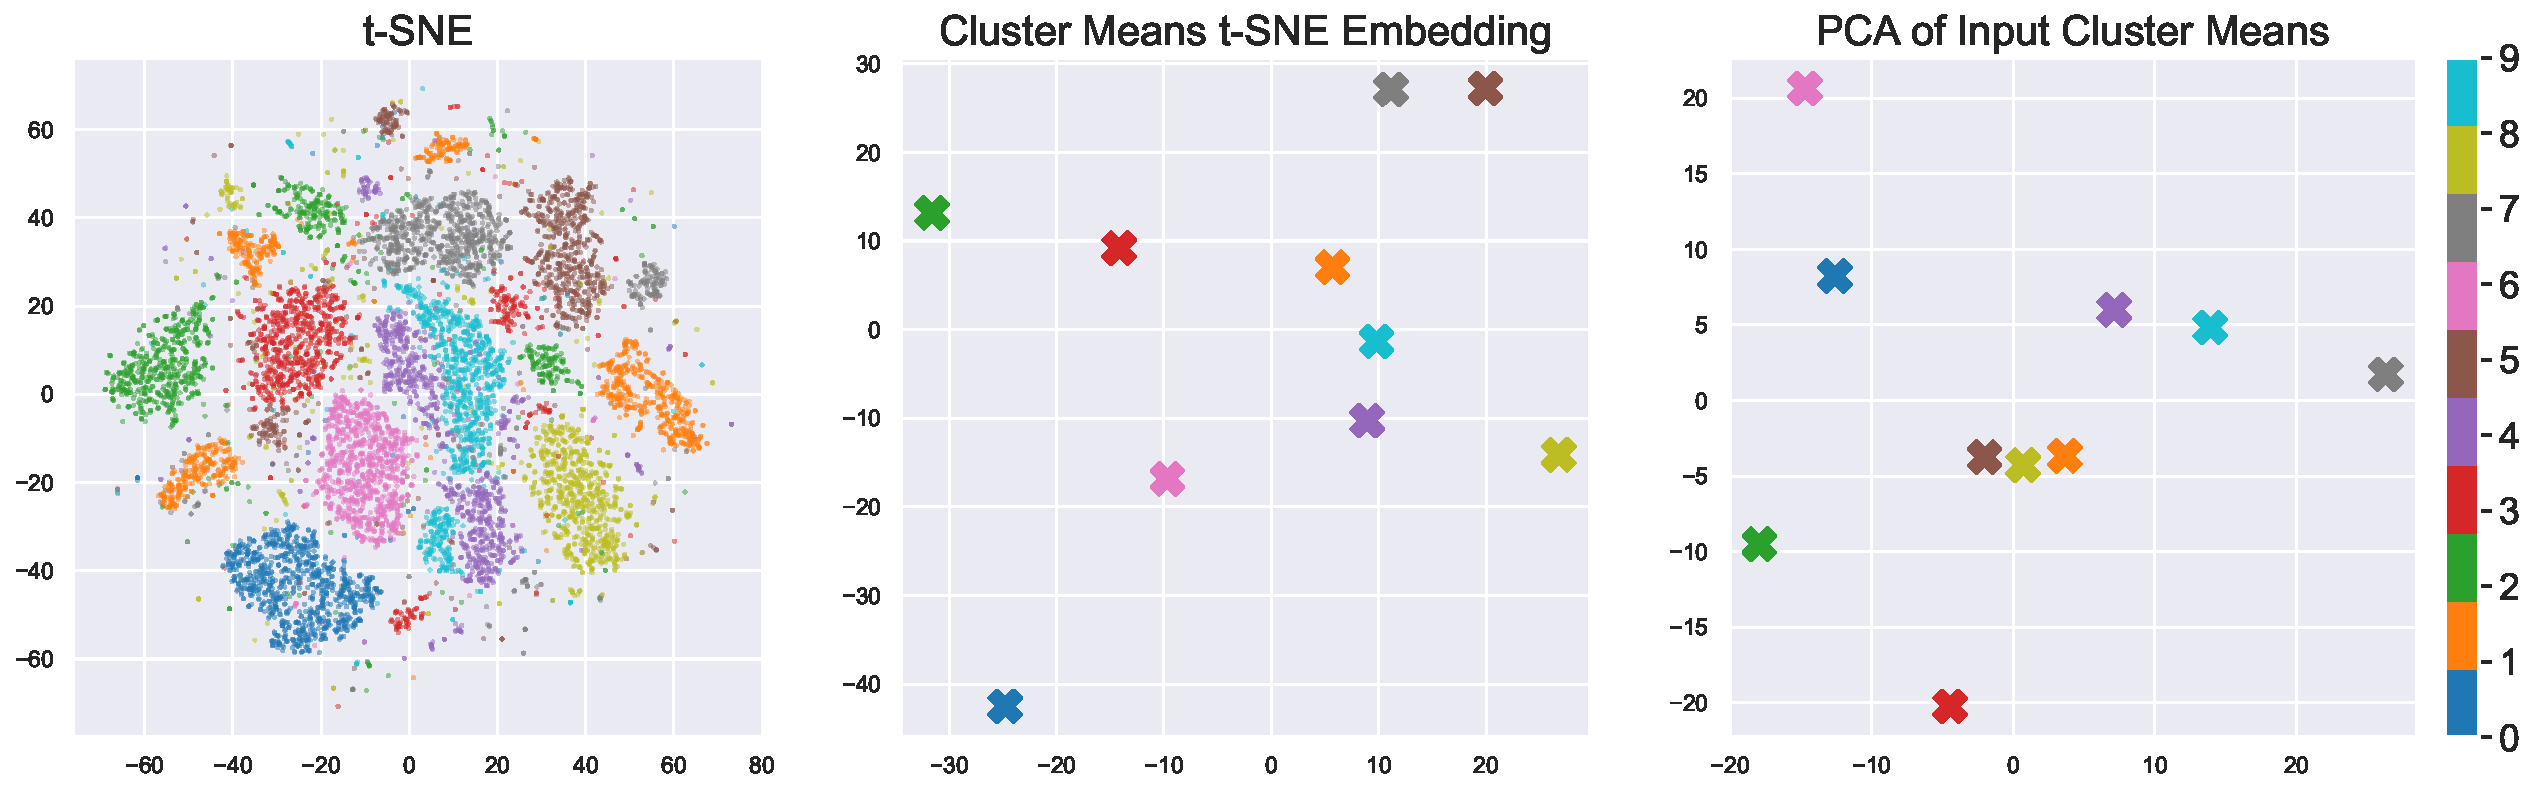
\includegraphics[width=0.5\columnwidth]{tSNE_truth.pdf}}
\caption{Left: MNIST t-SNE (perp : 30) embeddings initialized with i.i.d $\mathcal{N}(0,1)$ coordinates. Middle: using these t-SNE embeddings, mean coordinates for each digit are represented. Right: we compute a matrix of mean input coordinates for each of the $10$ digits and embed it using PCA. For t-SNE embeddings, the positions of clusters vary accross different runs and don't visually match the PCA embeddings of input mean vectors (right plot).}
\label{fig:tSNE-clusters-truth}
\end{center}
\end{wrapfigure}

\begin{corollary}\label{corollary_ccPCA}
Let $\W_{\scaleto{X}{4pt}} \in \mathcal{S}_{\scaleto{W}{4pt}}$, $\bm{L} = L(\overline{\W}_{\scaleto{X}{4pt}})$ and $\mathcal{S}^q_{\scaleto{M}{4pt}}= (\ker \bm{L}) \otimes \mathbb{R}^q$, then for all $\varepsilon > 0$, given the above hierarchical model, the solution of the problem:
$$\min_{\Z \in \mathcal{S}^q_{M}} \: -\mathbb{E}_{\bm{\Theta}_{\scaleto{X}{3pt}}| \X}\left[ \log \mathbb{P}(\bm{\Theta}_{\scaleto{Z}{4pt}} = \bm{\Theta}_{\scaleto{X}{4pt}}| \W_{\scaleto{Z}{4pt}} = \W_{\scaleto{X}{4pt}}, \Z) \right]$$
is a PCA embedding of $\bm{U}_{\scaleto{[:R]}{5pt}}\bm{U}_{\scaleto{[R]}{5pt}}^\top\X$ where $\bm{U}_{\scaleto{[:R]}{5pt}}$ are the CCs' membership vectors of $\overline{\W}_{\scaleto{X}{4pt}}$.
\end{corollary}

\begin{remark}
Note that while (\ref{eq:loss_LW}) approximates the objective of SNE-like methods when $\varepsilon \to 0$, the minimizer of (\ref{eq:add_term_Coupling}) given by \cref{corollary_ccPCA} is stable for all $\varepsilon$.
\end{remark}

From this observation, we propose a simple heuristic to minimize (\ref{eq:add_term_Coupling}) that consists in computing a PCA embedding of $\mathbb{E}_{\mathbb{P}_{\scaleto{\mathcal{P}_X}{4pt}}(\cdot;\bm{K}_{\scaleto{X}{3pt}})}\left[ \bm{U}_{\scaleto{[:R]}{5pt}}\bm{U}_{\scaleto{[R]}{5pt}}^\top \right]\X$. The distribution of the connected components of the posterior of $\W_{\scaleto{X}{4pt}}$ being intractable, we resort to a Monte-Carlo estimation of the above expectation. The latter procedure called \textit{ccPCA} aims at recovering the inter-CC structure that is filtered by SNE-like methods. \textit{ccPCA} may then be used as initialization for optimizing (\ref{eq:loss_LW}) which is done by running the DR method corresponding to the graph priors at hand (\cref{sec:retrieving_DR_methods}). This second step essentially consists in refining the intra-CC structure. 

\subsection{Experiments with \textit{ccPCA}}\label{sec:ccPCA}

\begin{figure*}[t]
\begin{center}
\centerline{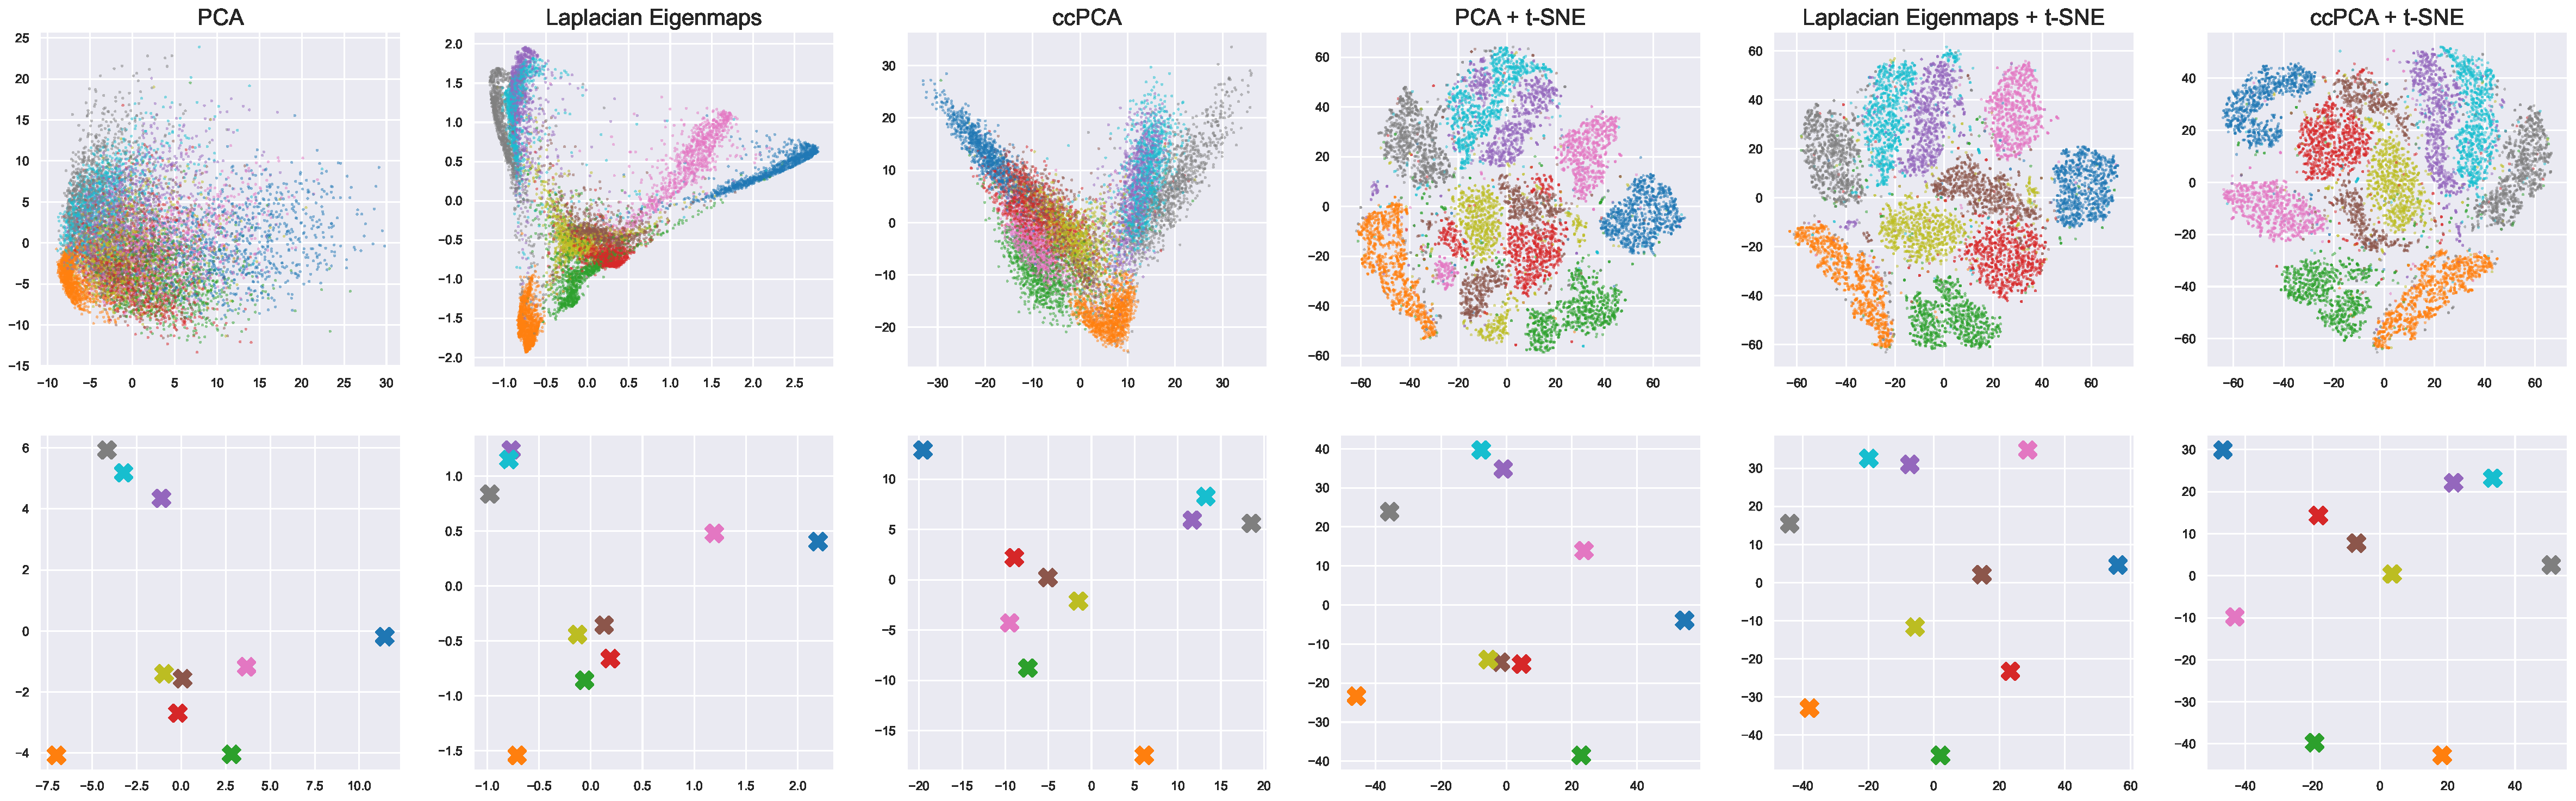
\includegraphics[width=\columnwidth]{cluster_positions.pdf}}
\caption{Top: MNIST embeddings produced by PCA, Laplacian eigenmaps, \textit{ccPCA} and finally t-SNE launched after the previous three embeddings to improve the fine-grain structure. Bottom: mean coordinates for each digit using the embeddings of the first row. The color legend is the same as in \cref{fig:tSNE-clusters-truth}. t-SNE was trained during $1000$ iterations using default parameters with the openTSNE implementation \cite{polivcar2019opentsne}.}
\label{fig:methods_embeddings}
\end{center}
\vspace{-0.8cm}
\end{figure*}

\Cref{fig:tSNE-clusters-truth} shows that a t-SNE embedding of a balanced MNIST dataset of 10000 samples \cite{deng2012mnist} with isotropic Gaussian initialization performs poorly in conserving the relative positions of clusters. As each digit cluster contains approximately $1000$ points, with a perplexity of $30$, sampling an edge across digit clusters in the graph posterior $\mathbb{P}_{\scaleto{\mathcal{P}_X}{4pt}}(\cdot;\bm{K}_{\scaleto{X}{4pt}})$ is very unlikely. Recall that the perplexity value \cite{maaten2008tSNE} corresponds to the approximate number of effective neighbors of each point. Hence images of different digits are with very high probability in different CCs of the graph posterior and their CC-wise means are not coupled as discussed in \cref{sec:interpretations}. To remedy this in practice, PCA or Laplacian eigenmaps are usually used as initialization \cite{kobak2021initialization}. 

These strategies are tested (\cref{fig:methods_embeddings}) together with \textit{ccPCA}. This shows that 
\textit{ccPCA} manages to retrieve the digits that mostly support the large-scale variability as measured by the peripheral positioning of digits $0$ (blue), $2$ (green), $6$ (pink) and $7$ (grey) given by the right side of \cref{fig:tSNE-clusters-truth}. Other perplexity values for \textit{ccPCA} are explored in appendix \ref{sec:other_perp} while the experimental setup is detailed in appendix \ref{sec:setup_exp}. In appendix \ref{sec:quantitative_evaluation}, we perform quantitative evaluations of \textit{ccPCA} for both t-SNE and UMAP on various datasets using K-ary neighborhood criteria. We find that using \textit{ccPCA} as initialization is in general more reliable than PCA and Laplacian eigenmaps for preserving global structure using both t-SNE and UMAP. 

Compared to PCA, \textit{ccPCA} manages to aggregate points into clusters, thus filtering the intra-cluster variablity and focusing solely on the inter-cluster structure. Compared to Laplacian eigenmaps which performs well at identifying clusters but suffers from the same deficiency as t-SNE for positioning them, \textit{ccPCA} retains more of the coarse-grain structure. These observations support our unifying probabilistic framework and the theoretical results about the MRF degeneracy which are the leading contributions of this article. The \textit{ccPCA} initialization appears as a first stepping stone towards more grounded DR methods based on the probabilistic model presented in this article.

\section{Conclusion and Perspectives}\label{Perspectives}

In this work we shed a new light on most popular DR methods by showing that they can be unified within a common probabilistic model in the form of latent Markov Random Fields Graphs coupled by a cross entropy. The definition of such a model constitutes a major step towards the understanding of common dimension reduction methods, in particular their structure preservation properties as discussed in this article. 

Our work offers many perspectives, among which the possibility to enrich the probabilistic model with more suited graph priors. Currently considered priors are simply the ones that are conjugate to the MRFs thus they are mostly designed to yield a tractable coupling objective. However they may not be optimal and could be modified to capture targeted features, \textit{e.g.}\ communities, in the input data, and give adapted representations in the latent space. The graph coupling approach could also be extended to more general latent structures governing the joint distribution of observations.
Finally, the probabilistic model could be leveraged to tackle hyper-parameter calibration, especially kernel bandwidths that have a great influence on the quality of the representations and are currently tuned using heuristics with unclear motivations. 
%\include{Chapters/Chapter3}
%\include{Chapters/Chapter4} 
%\include{Chapters/Chapter5} 

%----------------------------------------------------------------------------------------
%	THESIS CONTENT - APPENDICES
%----------------------------------------------------------------------------------------

\appendix % Cue to tell LaTeX that the following "chapters" are Appendices

% Include the appendices of the thesis as separate files from the Appendices folder
% Uncomment the lines as you write the Appendices

% Appendix A

\chapter{Frequently Asked Questions} % Main appendix title

\label{AppendixA} % For referencing this appendix elsewhere, use \ref{AppendixA}

\section{How do I change the colors of links?}

The color of links can be changed to your liking using:

{\small\verb!\hypersetup{urlcolor=red}!}, or

{\small\verb!\hypersetup{citecolor=green}!}, or

{\small\verb!\hypersetup{allcolor=blue}!}.

\noindent If you want to completely hide the links, you can use:

{\small\verb!\hypersetup{allcolors=.}!}, or even better: 

{\small\verb!\hypersetup{hidelinks}!}.

\noindent If you want to have obvious links in the PDF but not the printed text, use:

{\small\verb!\hypersetup{colorlinks=false}!}.

%\include{Appendices/AppendixB}
%\include{Appendices/AppendixC}

%----------------------------------------------------------------------------------------
%	BIBLIOGRAPHY
%----------------------------------------------------------------------------------------

\printbibliography[heading=bibintoc]

%----------------------------------------------------------------------------------------

\end{document}  
